\documentclass[11pt]{article}
\usepackage[english,magyar]{babel}
\usepackage{graphicx}
\usepackage{xcolor}
\usepackage[left=2.5cm, right=2.5cm]{geometry}
\usepackage{float}
\usepackage{hyperref}
\hypersetup{
	colorlinks=true,
	linkcolor=black,
	citecolor=blue,
	filecolor=magenta,      
	urlcolor=cyan,
	pdftitle={WaveFunctionSimulation},
	pdfpagemode=FullScreen,
}
\usepackage[acronym]{glossaries}
\usepackage{amsmath}
\usepackage{algorithm}
\usepackage{algpseudocode}
\usepackage{physics}
\usepackage{array}
\usepackage{subfig}


\urlstyle{same}
\bibliographystyle{IEEEtran}

%-------------------------------------------------------
% Custom commands:

\newcommand\todo[1]{
\begin{LARGE}
	\textcolor{red}{TODO: #1}\\
\end{LARGE}
}

\newcommand{\probP}{\text{I\kern-0.15em P}}

%-------------------------------------------------------


\title{Time evolution simulation of the quantum mechanical wave function in 3D space}
\author{Zoltán Simon\\[1cm]{\small Advisors: Dr. Balázs Csébfalvi, Dr. Géza István Márk, Dr. Péter Vancsó}}

\makeglossaries
\newacronym{qm}{QM}{Quantum Mechanics}
\newacronym{gr}{GR}{General Relativity}
\newacronym{dft}{DFT}{Discrete Fourier transform}
\newacronym{fft}{FFT}{Fast Fourier Transform}
\newacronym{gpu}{GPU}{Graphical Processing Unit}
\newacronym{cpu}{CPU}{Central Processing Unit}
\newacronym{fdtd}{FDTD}{Finite Difference in Time Domain}
\newacronym{fdtdq}{FDTD-Q}{FDTD technique for the analysis of quantum devices}
\newacronym{rkhofdtd}{RK-HO-FDTD}{Runge-Kutta High-Order Finite Difference in Time Domain}
\newacronym{api}{API}{Application Programming Interface}
\newacronym{cuda}{CUDA}{Compute Unified Device Architecture}
\newacronym{toml}{TOML}{Tom's Obvious Minimal Language}
\newacronym{brdf}{BRDF}{Bidirectional Reflectance Distribution Function}
\newacronym{wp}{WP}{Wave Packet}
\newacronym{wpd}{WPD}{Wave Packet Dynamics}
\newacronym{jit}{JIT}{Just In Time compilation}



\begin{document}
	\selectlanguage{english}
	
	\maketitle
		
	\begin{figure}[H]
		\centering
		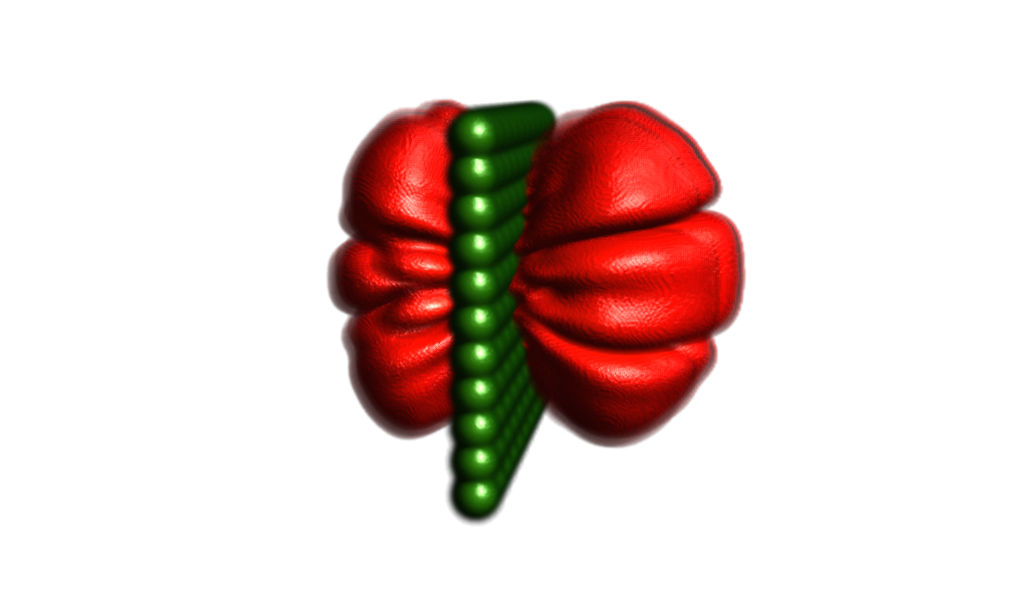
\includegraphics[width=0.75\textwidth]{figures/title_image.png}
	\end{figure}
	\thispagestyle{empty}
	\pagebreak
	\pagenumbering{arabic}
	
	\tableofcontents
	
	\pagebreak

	\section*{Abstract}

In quantum mechanics, the wave function describes the state of a physical system. In the non-relativistic case, the time evolution of the wave function is described by the time-dependent Schrö\-din\-ger equation. In 1982, D Kosloff and R Kosloff proposed a method \cite{KOSLOFF198335} to solve the time-dependent Schrödinger equation efficiently using Fourier transformation.
%Injected part:
The computational physics research group, led by Géza I. Márk in the
Nanotechnology Departement, Institute for Technical Physics and
Materials Science, Centre for Energy Research, in collaboration with
Belgian researchers developed a simulation method based on
three-dimensional wave packet dynamics for the study of the electron
dynamics in nanosystems. A simplified, interactive two-dimensional
version for educational purposes was published in 2020 \cite{mark2020webschrodinger}. In this
work, we demonstrate two improvements of the wave packed dynamical
simulation software: (i) the use of \acrfull{gpu},
which results in a vast (up to 50x) increase in simulation speed, and (ii)
the introduction of advanced visualization techniques \cite{raytracing_weekend, csebfalvi2023} which
are important to correctly interpret huge 4D space-time wave function
data sets obtained from the simulation.
%End of injected part
%In 2020, Géza István Márk published a paper \cite{mark2020webschrodinger} describing a computer program for the interactive solution of the time-dependent and stationary two-dimensional (2D) Schrödinger equation. Some details of quantum phenomena are only observable by calculating with all three spatial dimensions. We found it worth stepping out from the two-dimensional plane and investigating these phenomena in three dimensions. We implemented the above method for the three-dimensional case to simulate the time evolution of the wave function.
We used our implementation to simulate typical quantum phenomena using wave packet dynamics. First, we tried the method on analytically describable cases, such as the simulation of the double-slit experiment, and then we investigated the operation of flash memory. We used raytraced volumetric visualization to render the resulting probability density. In our work, we introduce the basics of wave packet dynamics in quantum mechanics. We describe the used method in detail and showcase our simulation results.\\
For further information and animations, please visite\\ \url{https://zoltansimon.info/src/content/research/wavepacketsim.html}

%\selectlanguage{magyar}
%\section*{Kivonat}
%
%A kvantummechanikában a hullámfüggvény írja le egy fizikai rendszer állapotát. Nemrelativisztikus esetben a hullámfüggvény időbeli fejlődését az időfüggő Schrödinger-egyenlet határozza meg. 1982-ben D Kosloff és R Kosloff közölt egy módszert \cite{KOSLOFF198335} az időfüggő Schrödinger-egyenlet hatékony megoldására Fourier-transzformáció felhasználásával. 2020-ban Márk Géza István cikkében \cite{mark2020webschrodinger} bemutatott egy interaktív szá\-mí\-tó\-gé\-pes programot az időfüggő és a stacionárius kétdimenziós Schrödinger-egyenlet megoldására. A kvantumos jelenségek bizonyos részletei csak mindhárom térdimenzióval számolva figyelhetők meg. Érdemesnek tartottuk a síkból kilépve, térben is megvizsgálni ezeket a jelenségeket. Munkánkban háromdimenziós esetre implementáltuk az említett módszert, hogy szimuláljuk a hullámfüggvény időbeli fejlődését. Hullámcsomag-dinamikát használva kipróbáltuk több jellegzetes kvantumos jelenség szimulációját. A módszert először analitikusan kezelhető esetekre teszteltük, például a kétréses kísérlet szimulációjára, ezután megvizsgáltuk a flash memória cella működését. A szimuláció kimeneteként előálló valószínűségi sűrűséget sugárkövetéses térfogati megjelenítéssel ábrázoltuk. Dolgozatunkban ismertetjük a kvantummechanikai hullámcsomag-dinamika alapjait. Részletesen leírjuk a használt eljárást, és bemutatjuk a szimulációnk eredményeit.\\
%További információ és animációk találhatóak a\\ \url{https://zoltansimon.info/src/content/research/wavepacketsim.html} webcímen.
%
%\selectlanguage{english}


	\pagebreak
	
	\section{Introduction}

In the first quarter of 20th century \acrfull{qm} opened a whole new window to understand our universe. Tamás Geszti in his book \cite{geszti2007} writes: learning \acrshort{qm} is part of the process of understanding the world, and the person who masters it, understands the world better.
It is a common view that while Albert Einstein's \acrfull{gr} provides a model that accurately describes the laws of nature governing large scale phenomena \cite{wald2010general}, quantum theory excels at atomic scale.
Although humanity has not yet accepted a single theory that would be capable of modeling both the small and large thus bridging the gap between \acrshort{qm} and \acrshort{gr}, there are many use-cases, where technology heavily depends on both theories.
\acrshort{qm} can be used efficiently to model the behavior of atomic particles.
It describes how electrons behave in the orbitals around atomic core and give an explanation for chemical reactions.
It can be used to model the structure of molecules.
\acrshort{qm} made possible for humanity the make use of the nuclear energy in power plants thus creating a new and efficient source of power.
Computers --as we know them today-- wouldn't be possible without a deep understanding of various quantum phenomena.
These systems make use of transistors \cite{Ross1998} which can also be thought of as a product of \acrshort{qm}.
In nanotechnology it is crucial to make quantum mechanical calculations to predict --and in many cases explain-- the behavior of different nanostructures.
One interesting field of study is the science of single-layer materials \cite{Zhuang2014}. These are also known as 2D materials.
One such carbon structure is called graphene \cite{VANCSO2013101, Márk2016}.
This single-layered structure conducts heat and electricity very efficiently thus raises high hopes in many when it comes to possible use-cases.
Nowadays quantum information science is getting larger and larger audience \cite{imresandor2004}.
Quantum Computing promises newer before seen increase in computation capabilities due to the massively parallel nature of quantum systems leveraging quantum superposition. Quantum Communication on the other hand opens new possibilities when it comes to secure information exchange with efficient channel encoding.
Although both of the last two fields mentioned await technological evolution in order to be commercially deployable due to a large amount of technical challenges, they both show that \acrshort{qm} has a lot of real life applications and the spectrum of these will only become more colorful as technology evolves.

Inspired by the previously enumerated large amount of various fields of application we targeted the goal to recreate the behavior of quantum systems in a computer simulation.
Such simulations are very useful for scientists. They use such methods to accurately model interaction between particles and various potential fields.
In order to accomplish this goal we choose a method that uses the \acrfull{fft} to efficiently calculate the time development of the quantum mechanical wave function.
In \acrshort{qm}, the wave function describes the state of a physical system. In the non-relativistic case, the time evolution of the wave function is described by the time-dependent Schrödinger equation \cite{schrodinger1926}.
In 1982, D Kosloff and R Kosloff proposed a method \cite{KOSLOFF198335} to solve the time-dependent Schrödinger equation efficiently using Fourier transformation.
In 2020, Géza István Márk published a paper \cite{mark2020webschrodinger} describing a computer program for the interactive solution of the time-dependent and stationary two-dimensional (2D) Schrödinger equation.
Some details of quantum phenomena are only observable by calculating with all three spatial dimensions.
We found it worth stepping out from the two-dimensional plane and investigating these phenomena in three dimensions.
Not that Géza István Márk and his colleagues have not already used 3D calculations in their research work.
The difference is that their implementation uses solely the \acrfull{cpu} of a computer.
For visualization of the resulting probability density so far they used isosurface method.
Our contribution mainly lays in leveraging the parallelisation potential of the modern \acrfull{gpu} thus significantly boosting the speed of the calculation by approximately a factor of 50 on our test hardware.
We also apply state of the art volumetric visualization techniques to create pleasing and comprehensible visuals for analysis of the evolution of probability density in 3D space.
We believe that by combining the knowledge available for computer visualization specialists and physicists we can arrive to something greater than the possibilities available if each of us would be working only in his or her own domain of expertise.
We write our implementation with future extendibility in mind, since we would like to continue our work and develop a capable simulation platform that can be deployed as a tool for state of the art scientific research.

In section \ref{sec:theory} of this article we start by discussing the theoretical background.
Then in section \ref{sec:used_method} we proceed to describe the used Fourier method to simulate the wave function.
In section \ref{sec:our_implementation} we provide an overview of the implementation details of our program.
After this in section \ref{sec:results} we showcase our simulation results.
Here we compare analytically describable simulation cases to the mathematical model.
At the end in section \ref{sec:discussion} we summarize our results in a short discussion.






	
	\section{Theoretical background}
\label{sec:theory}

\subsection{Beginnings of quantum mechanical wave dynamics}

In this section, we would like to give a brief introduction to the theory of \acrshort{qm}. In this summary of physics history, we rely mainly on Tamás Geszti's \acrshort{qm} book \cite{geszti2007}.
For English literature, we would like to point the reader's attention towards the critically acclaimed book of Claude Cohen-Tannoudji et al. \cite{tannoudjiVol1}.
%We will start our introduction with Max Planck.
%He gave an explanation for the drop in the spectrum of black-body radiation for high frequencies with constant temperature.
%He argued that each harmonic oscillator can only obtain energy in discrete energy elements of
%\begin{equation}
%	\label{eq:energy_quantum}
%	E_\delta = h\nu
%\end{equation}
%where $h$ is called the Planck constant and equals to $h = 6,6 \times 10^{-34}\;Js$
%and $\nu$ is the frequency of the oscillator.
%For convenience physicists tend to use $\hbar = \frac{h}{2\pi}$ reduced Planck constant.
%With this equation \ref{eq:energy_quantum} can be written in the form of
%\begin{equation}
%	E_\delta = \hbar\omega
%\end{equation}
%
%At this point, it was known to physicists that a black body can be modeled with electromagnetic harmonic oscillators with different modes that satisfy the boundary conditions of the box. Consequently, Planck was able to give a formula that accurately models the energy emission of black-bodies.
%The next advancement was in 1905, when Albert Einstein explained the photoelectric experiment.
%This experiment was first performed and documented by Fülöp Lénárd resulting in a Nobel prize for him.
%This experiment demonstrates that electrons can exit a metal electrode only by shining light on it.
%Here an important observation was made, which can be described by saying that the $E_{photo}$ energy of exited electron only depends on the color of light shining on the electrode.
%Einsteins discovery can be formally written in the following equation
%\begin{equation}
%	E_{photo} = h\nu - W
%\end{equation}
%where $W$ is the work required for the electron to leave the electrode.
%This is the second time the Planck constant appears in a physical formula.
%It suggests that the electron absorbs the energy of one single light quantum (photon, as we would call today).
%
%Ernest Rutherford experimented with shooting high energy positively charged $\alpha$-particles into materials and observing the refraction of these particles.
%He came to the conclusion that the largest portion of the mass of the materials is clumped into heavy positively charged cores and light negatively charged electrons surround the positive cores.
%According to his explanation the reason why these negatively charged particles do not fall into the positive core is that they orbit the core similarly to how planets do orbit the Sun.
%This however results in a paradox.
%Negatively charged orbiting particles should emit electromagnetic radiation thus quickly loosing energy and consequently falling into the core.
%
%Physicist have examined the color spectrum of atomic gases such as hydrogen.
%They observed that such gases exhibit a spectrum of discrete lines.
%To explain this strange phenomena in 1913, Niels Bohr made the connection between Planck's energy quantum hypothesis and Einstein's photon hypothesis.
%He stated that the electrons orbiting the atomic core occupy only orbitals with certain energy levels, and somehow evade the continuous transition between these orbitals.
%When they do make the transition between the discrete energy levels of $E_n$ and $E_m$ they emit or absorb photons based on whether they gained or lost energy.
%\begin{equation}
%	h\nu = E_m - E_n
%\end{equation}


In 1924, Louis de Broglie recognized that an electron moving with momentum of $p=M_ev$ can also be thought of as the propagation of some kind of a matter wave with $\lambda$ wavelength.
\begin{equation}
	\label{eq:de_broglie}
	\lambda = \frac{h}{p}
\end{equation}
where $h$ is called the Planck constant and equals to $h = 6,6 \times 10^{-34}\;Js$.
This also explains the discrete energy levels in Bohr's model.
The allowed orbitals are those where the wave is a single-valued function and thus closes into itself after one full rotation of $2\pi$ radians.
If we use polar coordinates, this means that the wave has the same complex amplitude for coordinates $\alpha$ and $\alpha + n2\pi$ where $n = 0, 1, 2, \dots$.
Here we can further modify equation \ref{eq:de_broglie} and arrive to
\begin{equation}
	\vec{p} = \hbar \vec{k}
\end{equation}
where $\vec{k}$ is the wave vector and $\hbar = \frac{h}{2\pi}$ is the reduced Planck constant.
The amplitude of this vector equals $\|\vec{k}\|= \frac{2\pi}{\lambda}$, and its direction is perpendicular to the wavefront.

Experiments show that matter waves exhibit self-interfering behavior similar to electromagnetic waves\footnote{An electron always only interferes with itself while light waves coming from multiple light sources can also interfere with each other.}.
For example, the double-slit experiment, where a wave propagates through a barrier with a pair of two narrow slits and consequently creates an interference pattern on a canvas placed after the barrier, can be performed not only with light but a single electron as well.
When the experiment is performed with electrons, the canvas is replaced with a measurement device that is able to register the incoming electron.
By performing this experiment once, the measuring device will only register the electron at a single location.
The interference becomes noticeable only after repeating the measurement multiple times since the distribution of the measured electron impact locations converges to the interference pattern.
This behavior is also referred to as wave–particle duality because the particle interferes with itself, but also, there is only one single impact at the measuring device for each iteration of the experiment.
Another important experimental observation is that if we create the linear combination of multiple matter waves and then the combined wave evolves over time than the resulting wave is precisely the same as if the originally combined waves would have evolved independently and we would only have combined the resulting waves.
This latter property was also true for electromagnetic waves, and its called the superposition principle.
Please note that although we keep comparing electromagnetic waves with matter waves, the two are different phenomena.
One significant difference is that interference of electromagnetic waves happen due to different strength of electric and magnetic fields.
In \acrshort{qm} the wave function has a complex value thus, it can interfere even when only the phase is different and the amplitude is the same.
Our goal in emphasizing the similarities is only to reinforce a possible intuition in those perhaps more familiar with the world of electromagnetism.

\subsection{Wave packet dynamics}

Erwin Schrödinger introduced the concept of the \acrfull{wp} to show that in limiting cases \acrshort{qm} gives back the classical particle model where small bullets are moving around and colliding.
This particle-like propagation of a \acrshort{wp} of the wave is due to the superposition of waves with different frequencies forming peaks.
These waves extinguish each other for the most part, but at some position and time coordinates, the amplitudes add up to larger amplitude.
An example of this is demonstrated in figure \ref{fig:superposition}.
\begin{figure}[hbt!]
	\centering
	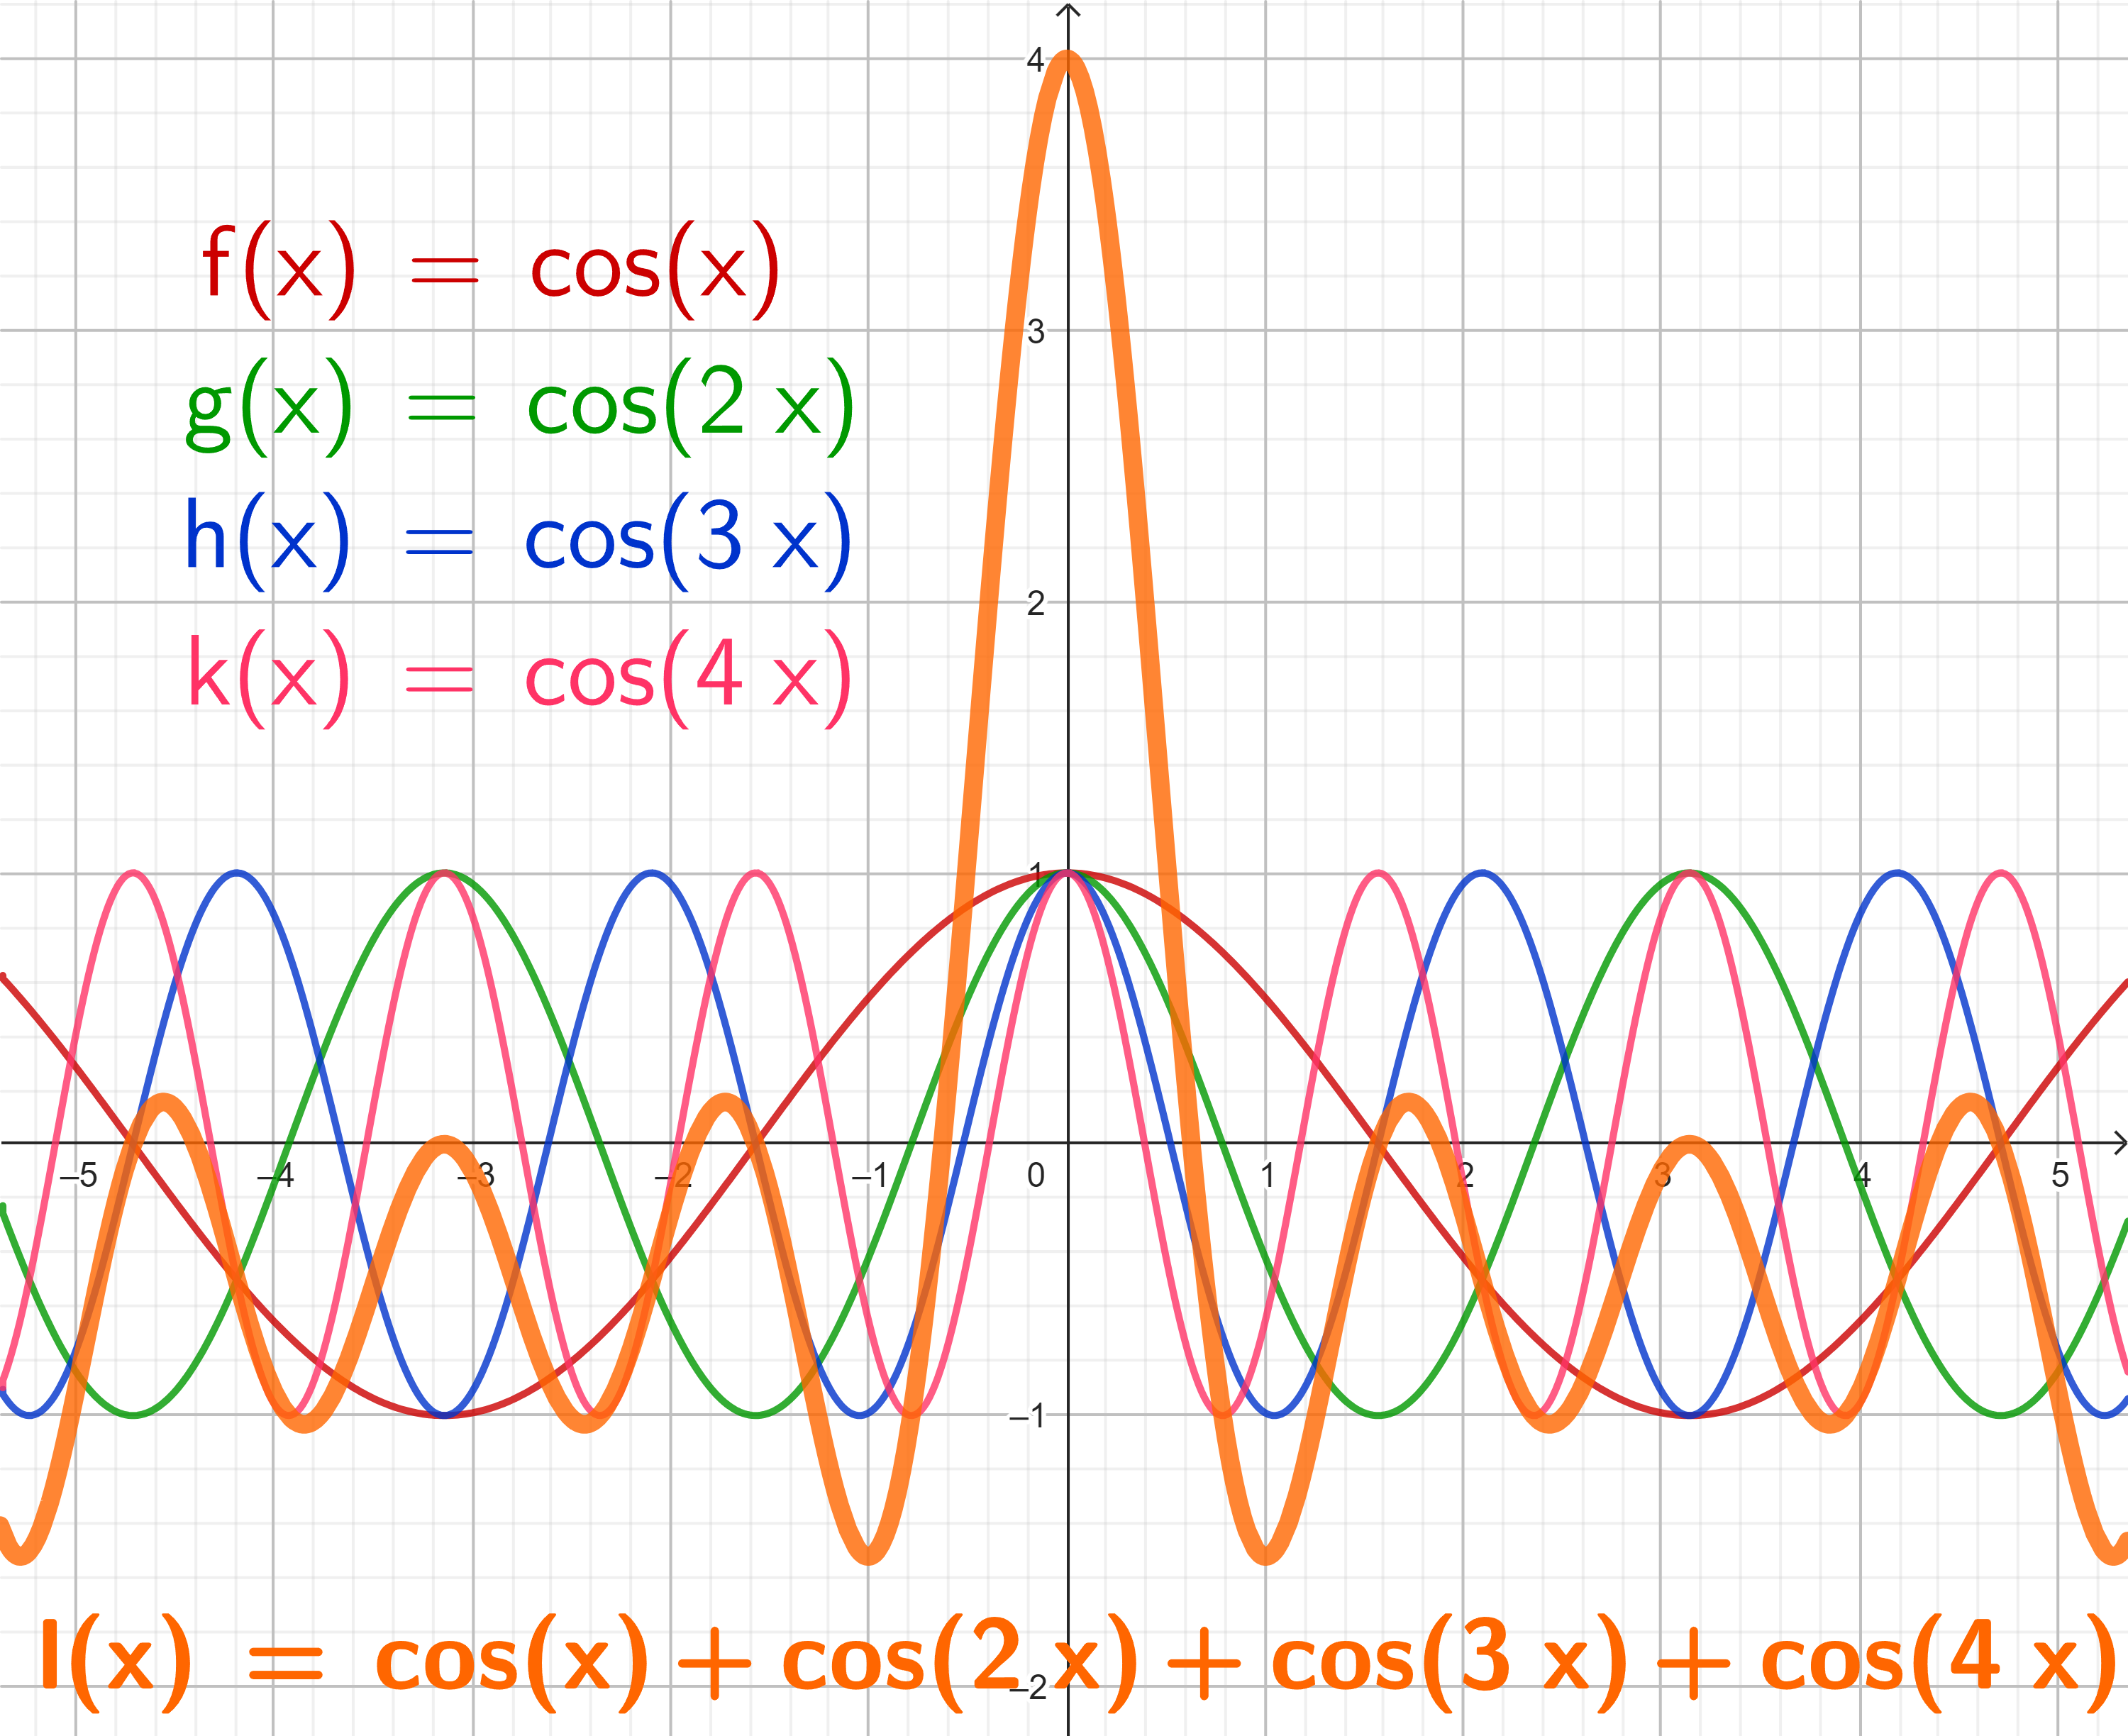
\includegraphics[width=0.5\textwidth]{figures/Superposition of cosine waves.png}
	\caption{Superposition of cosine waves with different wavelength: the superposition forms a peak at the $x = 0$ coordinate}
	\label{fig:superposition}
\end{figure}

$\Psi_k$ denotes the complex amplitude of a matter wave with $k=\frac{2\pi}{\lambda}$ wave number. The formula of a plane wave propagating in positive $x$ direction can be described in the form of equation \ref{eq:plane_wave_k}.

\begin{equation}
	\label{eq:plane_wave_k}
	\Psi_k(x, t) = e^{i(kx - \omega t)}
\end{equation}

Let's calculate the superposition of waves with different wave numbers! We assume that the angular velocity $omega(k)$ depends on the $k$ wave number and that the waves with different wave numbers have various $c(k)$ weights in the linear combination. This gives the following Fourier integral:
\begin{equation}
	\label{eq:combination_of_waves}
	\Psi(x, t) = \int_k c(k) sin[kx - \omega(k)t]\; dk
\end{equation}

By analyzing this formula, we can determine the propagation velocity of the amplitude peaks.
In equation \ref{eq:combination_of_waves}, the peaks form where and when the phase of the sine function is not dependent on the $k$ integration variable. In other words, the derivative of the phase with respect to $k$ is zero.
\begin{equation}
	\label{eq:derivative_of_phase}
	\frac{d}{dk}[kx - \omega(k)t] = x - \frac{d}{dk}\omega(k)t = 0
\end{equation}

By generalizing for all spatial coordinates and rearranging equation \ref{eq:derivative_of_phase}, we get the group velocity of the wave.
\begin{equation}
	\label{eq:group_velocity}
	\vec{v}_{group} = \frac{\delta \omega(\vec{k})}{\delta \vec{k}}
\end{equation}
By using the $E := \hbar \omega$ and $\hbar \vec{k} = \vec{p}$ substitutions for the energy and momentum, we arrive at the classically known formula for a particle of mass $m$
\begin{equation}
	\label{eq:classical_group_velocity}
	\vec{v}_{group} = \frac{\delta E(\vec{p}, \vec{r})}{\delta\vec{p}} = \frac{\delta}{\delta\vec{p}}\left[ \frac{\|\vec{p}\|^2}{2m} + V(\vec{r}) \right] = \frac{\vec{p}}{m}
\end{equation}
There are, however significant differences between the classical and \acrshort{qm} model.
The particle analogy comes with its limits.
In 1927, Werner Heisenberg formulated his uncertainty principle.
This states that simultaneously, the position and the momentum of a particle can not be determined precisely.
Only with a specific $\Delta$ precision.
The result can be written in the form of equation \ref{eq:heisenberb_uncertainty}.
\begin{equation}
	\label{eq:heisenberb_uncertainty}
	\Delta x \cdot \Delta p \geq \frac{\hbar}{2}
\end{equation}
A similar relation holds between time and energy.
\begin{equation}
	\label{}
	\Delta t \cdot \Delta E \geq \frac{\hbar}{2}
\end{equation}

\subsection{The Schrödinger equation}

So far, we know that atomic particles exhibit wave-like behavior, and in bounded systems, they can absorb or release energy only in discrete quanta.
These matter waves can interfere with each other, and the superposition principle holds true.
Along the way, we obtained a seemingly satisfactory energy, momentum, and velocity concept.
One last step is to, instead of real amplitudes we allow complex amplitudes.
This solves the problem of energy conservation.

All of these advancements led up to the formalization of the Schrödinger equation in 1926 by Erwin Schrödinger \cite{schrodinger1926}.
Already in the 19th century, in the field of optics, it was common practice to use linear partial differential equations to calculate light propagation.
Linearity is a requirement for matter waves as well, since by the definition of superposition a general equation that aims to describe the behavior of matter waves adequately must be satisfied by the simple waves and also by the linear combination of these waves.
Let us write the $\Psi$ plane wave as a complex-valued function
\begin{equation}
	\Psi(\vec{r}, t) = e^{i(\vec{k}\cdot\vec{r} - \omega t)} = e^{\frac{i}{\hbar}(\vec{p}\cdot\vec{r} - Et)}
\end{equation}

First, let's assume that our wave is propagating in free space.
The total energy of the particle consists only of kinetic part.
\begin{equation}
	\label{eq:kinetic_energy}
	E=\frac{p^2}{2m}
\end{equation}
We don't know the equation for the wave function yet, but it must incorporate this relation between the energy and momentum.
In the wave function, both the energy and the momentum are in exponent.
To express them, we have to take the derivative of the function with respect to position and time.
The operation of calculating the partial derivative with respect to position is often referred to as calculating the gradient vector and is denoted by the $\nabla$ ("nabla") symbol.
\begin{equation}
	\label{eq:derivative_of_wave_func}
	\begin{split}
		\frac{d}{dt}\Psi(\vec{r}, t) &= -\frac{i}{\hbar}E\;\Psi(\vec{r}, t)\\
		\frac{\delta}{\delta\vec{r}}\Psi(\vec{r}, t) &= \nabla \Psi(\vec{r}, t) =	\frac{i}{\hbar}\vec{p}\;\Psi(\vec{r}, t)
	\end{split}
\end{equation}
In the kinetic energy equation \ref{eq:kinetic_energy}, we actually need the square of the magnitude of momentum.
To calculate it, we introduce the $\Delta = \vec{\nabla} \cdot \vec{\nabla}$ Laplace operator.
By combining equation \ref{eq:kinetic_energy} and \ref{eq:derivative_of_wave_func} we can arrive to the following linear differential equation
\begin{equation}
	\label{eq:schrodinger_free_space}
	i \hbar \frac{d}{dt}\Psi(\vec{r}, t) = - \frac{\hbar^2}{2m}\Delta\Psi(\vec{r}, t)
\end{equation}
This is the Schrödinger equation for matter wave propagating in free space.
Let's generalize this by eliminating the previous assumption that the total energy is solely kinetic.
Now, we allow an $V(\vec{r})$ localized potential energy to be an arbitrary function of location. Thus, the total energy becomes
\begin{equation}
	\label{eq:hamilton_function}
	E = \frac{p^2}{2m} + V(\vec{r}) = \mathcal{H}(\vec{p}, \vec{r})
\end{equation}
Here, we introduced the $\mathcal{H}$ notation to express that this is a form of the so-called Hamiltonian function named after William Rowan Hamilton, who used his formalism to describe classical mechanics in the 19th century \cite{Hamilton1833}.
Using equation \ref{eq:hamilton_function} to modify equation \ref{eq:schrodinger_free_space}, we trivially arrive at the more general form of the Schrödinger equation
\begin{equation}
	\label{eq::schrodinger_general}
	\begin{split}
		i \hbar \frac{d}{dt}\Psi(\vec{r}, t) &= - \frac{\hbar^2}{2m}\Delta\Psi(\vec{r}, t) + V(\vec{r})\Psi(\vec{r}, t)\\
		\frac{d}{dt}\Psi(\vec{r}, t) &= -\frac{i}{\hbar}\hat{H}\Psi(\vec{r}, t)
	\end{split}
\end{equation}
We can see that on the left side, we basically take the first derivative of the wave function with respect to the time and on the right side we let a $\hat{H} = -\frac{\hbar^2}{2m}\Delta + V(\vec{r})$ operator affect the wave function.
By solving this differential equation and specifying an initial state, we can predict the time development of a quantum mechanical wave function.

The only remaining question also meaningful for our simulation is that how exactly should we interpret the resulting function?
What's the actual physical meaning behind the amplitude of the wave?
Experiments show that the square of the absolute value of the complex amplitude is the probability density associated with the particle being found in a given infinitesimally small portion of space at a given time.
For convenience and to be sound with probability theory, we normalize the amplitude of the wave function so that the velocity of the particle being found "somewhere" in space equals $\probP = 1$.
\begin{equation}
	\label{eq:normalization}
	\int_\mathcal{V} |\Psi(\vec{r}, t)|^2 \;d^3r = 1
\end{equation}



	
	\section{Used method}
\label{sec:used_method}

In our simulation we numerically solve the time dependent Schrödinger equation.
There are multiple available algorithms for this task.
A widely used category of solving strategies are the \acrfull{fdtd} methods.
This approach is also widely adopted to simulate the solution of Maxwell equations \cite{maxwell1865, Ulf2001}.
\acrfull{fdtdq} however exhibit numerical instability \cite{Soriano2004}.
After a longer sequence of simulation steps the solutions diverge from the ground truth.
There are various alterations of the base method.
One such method was proposed by Min Zhu et al. \cite{Zhu2014} in the year 2014.
Their algorithm is called the \acrfull{rkhofdtd}.
In 2021, a follow up paper \cite{Zhu_Wang_2021} demonstrated the superiority of \acrshort{rkhofdtd} over the basic \acrshort{fdtdq} approach.
In the same year Frederick Ira Moxley et al. \cite{MOXLEY20122434} proposed another method based on \acrshort{fdtdq}.
These methods solve the majority of problems related to \acrshort{fdtdq}.

However in our work we use a different approach.
Back in 1982, D Kosloff and R Kosloff proposed a method \cite{KOSLOFF198335} to solve the time-dependent Schrödinger equation efficiently using Fourier transformation.
The advantage of this algorithm is the high numerical stability of the time evolution step.
In the adopted \acrshort{fft} method no signs of divergence are present even after a large number of simulation steps.
The time development step of the algorithm has a time complexity of $\mathcal{O}(N\log N)$ since it only uses six \acrshort{fft} runs ($\mathcal{O}(N\log N)$ each) and three element wise multiplication between tensors ($\mathcal{O}(N)$ each).
The amount of \acrshort{fft} runs and multiplications can be reduced further if we don't want to read the results of the time development in each step.
A significant speed up can be reached by using parallelized implementation of the \acrshort{fft} algorithm as we did by using an efficient \acrshort{gpu} implementation.
In the following part we would like to explain the \acrshort{fft} method in detail.
Let's start by deriving the formal solution of the \ref{eq::schrodinger_general} differential equation.
\begin{equation}
	\label{eq:formal_solution}
	\begin{split}
		\int_{t_0}^t \frac{d}{d\tau}\Psi(\vec{r}, \tau) \; d\tau &= \int_{t_0}^t -\frac{i}{\hbar}\hat{H}\Psi(\vec{r}, \tau)\; d\tau\\
		\Psi(\vec{r}, t) - \Psi(\vec{r}, t_0) &= \int_{t_0}^t -\frac{i}{\hbar}\hat{H}\Psi(\vec{r}, \tau)\; d\tau\\
		&\;\:\vdots\\
		\Psi(\vec{r}, t) &= e^{-\frac{i}{\hbar}\hat{H}(t - t_0)} \Psi(\vec{r}, t_0)
	\end{split}
\end{equation}
where $\Psi(\vec{r}, t_0)$ is a specified initial state and $\Psi(\vec{r}, t)$ is the state after some $\delta t = t - t_0$ time.
The problematic part is the Hamiltonian operator in the exponent.
The kinetic and potential operators can not be commuted in general, hence exponential can not be factored.
Géza István Márk in his Web-Schrödinger simulator \cite{mark2020webschrodinger} decomposes the exponential by the symmetrical unitary product as shown in form \ref{eq:unitary_product}.
\begin{equation}
	\label{eq:unitary_product}
	e^{-\frac{i}{\hbar}\hat{H}\delta t} = e^{-\frac{i}{\hbar}(\hat{K} + \hat{V})\delta t} \approx e^{-\frac{i}{\hbar}\hat{K}\delta t / 2}\; e^{-\frac{i}{\hbar}\hat{V}\delta t}\; e^{-\frac{i}{\hbar}\hat{K}\delta t / 2}
\end{equation}
The error of this approximation is $\mathcal{O}(\delta t^3)$ therefore we have to be careful with the selection of small enough time resolution.
When the potential energy is localized the $\hat{V}$ operator is a simple multiplication with $V(\vec{r})$ function thus the middle part of the product is as follows
\begin{equation}
	\label{eq:potential_prop}
	e^{-\frac{i}{\hbar}\hat{V}\delta t} \Psi = e^{-\frac{i}{\hbar}V(\vec{r})\delta t} \Psi
\end{equation}
The $\hat{K}$ kinetic operator involves calculating the spatial derivative of the wave function.

Previously in equation \ref{eq:derivative_of_wave_func} we have seen that calculating the spatial gradient $\nabla \Psi(\vec{r}, t)$ yields multiplication by $\frac{i}{\hbar}\vec{p} = i\vec{k}$.
We only need to get the value of the wave vector.
This is when the Fourier transform comes into play which transforms between real space and momentum space.
Following relation holds for the derivative of an arbitrary $f$ function and it's Fourier transform
\begin{equation}
	ik\mathcal{F}\{f\} = \mathcal{F}\{f'\}
\end{equation}
Taking the derivative in real space means multiplication by $ik$ imaginary wave number in momentum space.
We work with the $\Delta = \nabla \cdot \nabla$ Laplace operator so we have to multiply by $(ik)^2 = -k^2$.
By exploiting the linearity of Fourier transform we arrive to the following formula for the kinetic energy part of the Hamiltonian function
\begin{equation}
	\label{eq:kinetic_op}
	\hat{K} \Psi = \frac{p^2}{2m}\Psi = -\frac{\hbar^2}{2m} \Delta \Psi = -\frac{\hbar^2}{2m}\mathcal{F}^{-1}
	\{
		-k^2\mathcal{F}\{\Psi\}
	\}
\end{equation}
where $\mathcal{F}^{-1}$ is the inverse Fourier transform. In momentum space the $k$ wave number is trivially given as it can be thought of as the very coordinate the functions are parameterized with.
Having that said, it is important to distinguish between $\nu$ frequency, $\lambda$ wavelength, $k$ wave number and even $\omega$ angular velocity.
These relate as follows
\begin{equation}
	\label{eq:relation_of_dimensions}
	k = \frac{2\pi}{\lambda} = \frac{2\pi\nu}{v_{group}} = \frac{\omega}{v_{group}}
\end{equation}
where $v_{group}$ denotes the group velocity of the wave.

Actually in equation \ref{eq:unitary_product} the $\hat{K}$ kinetic energy operator is in the exponent multiplied by $-\frac{i}{\hbar}\delta t / 2$.
Using the knowledge gathered from equation \ref{eq:kinetic_op} we can now write
\begin{equation}
	\label{eq:kinetic_prop}
	e^{-\frac{i}{\hbar}\hat{K}\delta t / 2}\Psi = \mathcal{F}^{-1}
	\left[
		e^{-\frac{i}{\hbar} \left(-\frac{\hbar^2}{2m}\right) \left(-k^2\right) \delta t / 2} \mathcal{F}\left[ \Psi \right]
	\right] = 
	\mathcal{F}^{-1}
	\left[
	e^{-\frac{i k^2 \hbar \delta t}{4m}} \mathcal{F}\left[ \Psi \right]
	\right]
\end{equation}

Before writing the pseudo code let's 
Let's write the wave function as a function of discrete $i_j \in \{0, 1, \dots, N_j - 1\}$ coordinates where $j \in \{x, y, z, t\}$ and $N_j$ are the number of discrete grid points along each axis.

Now $\vec{r}_x = i_x \delta x$, $\vec{r}_y = i_y \delta y$, $\vec{r}_z = i_z \delta z$ and $t = i_t \delta t$ are the original spatial and time coordinates and $\delta j$ is the resolution of the different dimensions respectively.
With the new discretized coordinates the Schrödinger equation \ref{eq::schrodinger_general} can be written in the following form
\begin{equation}
	\label{eq:discretized_schrodinger}		
	i \hbar \frac{d}{dt}\Psi(i_x, i_y, i_z, i_t) = - \frac{\hbar^2}{2m}\Delta\Psi(i_x, i_y, i_z, i_t) + V(\vec{r})\Psi(i_x, i_y, i_z, i_t)
\end{equation}
Having a discrete data set, \acrfull{dft} can be efficiently implemented using the \acrfull{fft} algorithm.
The output of simulation is the probability density for each --approximately infinitesimally small-- discrete grid cell.
This can be obtained by calculating the square of the absolute value of the wave function for each grid cell which is the same as calculating the standard scalar product between $\bra{\Psi}$ and $\ket{\Psi}$ vectors where $\bra{\Psi}$ is the transposed complex conjugate of $\ket{\Psi}$ as seen in equation~\ref{eq:probability_density}.
\begin{equation}
	\label{eq:probability_density}
	p(\vec{r}, t) = |\Psi(\vec{r}, t)|^2 = \braket{\Psi(\vec{r}, t)}
\end{equation}
Making use of formulas \ref{eq:unitary_product}, \ref{eq:potential_prop} and \ref{eq:kinetic_prop} and plugging them into the formal solution of the Schrödinger equation we can create an algorithm for the time development of the wave function.
We will use the $\Psi$ to represent a complex valued tensor where the elements of this tensor can be obtained by using the $i_j$ discrete indices.
The algorithm can be written in the form of the following pseudo code

\begin{algorithm}
	\caption{Time advance algorithm}\label{alg:time_advance}
	\begin{algorithmic}
		\State $ \Psi \gets $ initial state of the wave function
		\State $ V \gets $ localized potential
		\State $ \delta t \gets $ time resolution
		\State $ N_t \gets $ number of time steps
		\For{$i \in [0, N_t)$}
			\State $\Psi^{(1)} \gets FFT^{-1}
			\left[
			P_K\; FFT\left[ \Psi \right]
			\right]
			$
			
			\State $\Psi^{(2)} \gets P_V\; \Psi^{(1)}$
			
			\State $\Psi \gets FFT^{-1}
			\left[
			P_K\; FFT\left[ \Psi^{(2)} \right]
			\right]
			$
			\State Visualize $|\Psi|^2$
		\EndFor
	\end{algorithmic}
\end{algorithm}

Here $P_K(i_x, i_y, i_z) \sim e^{-\frac{i \hbar \delta t}{4m} \left[(2\pi i_x / N_x / \delta x)^2 + (2\pi i_y / N_y /\delta y)^2 + (2\pi i_z / N_z / \delta z)^2\right]}$ is the kinetic energy propagator in momentum space and $P_V(i_x, i_y, i_z) = e^{-\frac{i}{\hbar}V(i_x, i_y, i_z)\delta t}$ is the potential energy propagator in real space.
We used the discretized coordinates to express the same operations as in \ref{eq:potential_prop} and \ref{eq:kinetic_prop}.
Please note that in the kinetic propagator's case it is important to follow the convention used by the specific \acrshort{fft} implementation.
The formula written here is not entirely correct.
The \acrshort{fft} used in our implementation puts the amplitude associated with the largest representable frequency of $\frac{1}{2N}$ in the middle of the tensor.
In the second half of the tensor for each axis the amplitudes are for the negative frequencies in ascending absolute value so that the largest index represents the $-\frac{1}{N}$ frequency.
This means that we had to modify the definition of $P_K$ accordingly.
One way to make the correction is to check whether $i_j / N_j > \frac{1}{2}$ is true. If it is than modify it like $i_j := N - i_j$.

When working with \acrshort{dft} it is important to take into account the boundary conditions of the transformed region.
The \acrshort{dft} implies periodic boundary condition in which value at $i_j = 0$ connects smoothly to values at $i_j = 0$ for each of the respective $j \in \{x, y, z\}$ dimensions.
If the data transform does not satisfy this condition unrealistic artifacts arise.
One technique to battle this requirement is to define a high potential wall on all the edges of the simulated volume so that the wave packet bounces back and never reaches the problematic edge.
This however limits the possible simulation cases since we can not simulate scenarios where the wave packet would leave the volume.
The wave packet reflected by the boundary potential interferes with itself thus potentially disturbing the observation of the object of simulation.
In our implementation we used another approach called free space boundary condition.
This fixes the issues arising both with the periodic boundary condition and the potential box.
We extend the simulated volume beyond the observed part and outside the visible box we create a draining potential.
This draining potential gradually increases towards the edge of the simulated volume.
As the name suggests it's effect on the wave packet is that it diminishes it's amplitude.
By initializing a high enough draining potential the unrealistic artifacts on the edge of the simulated volume are practically negligible.
In equation \ref{eq:potential_prop} we have seen that the potential propagator is a multiplication by a unit length complex number with phase proportional to $V(\vec{r})$ localized potential.
This normally only introduces a rotation on the complex plane.
We can however incorporate the desired draining effect by introducing complex potential.
Let's examine what happens if a complex number has a complex phase!
\begin{equation}
	\label{eq:complex_phase}
	e^{i |z|e^{i\gamma}} = e^{i|z|\left[cos(\gamma) + isin(\gamma)\right]} = e^{i|z|cos(\gamma) - |z|sin(\gamma)}
	= e^{i|z|cos(\gamma)}e^{-|z|sin(\gamma)}
\end{equation}
In equation \ref{eq:complex_phase} We showed that by defining an imaginary potential we can reduce the magnitude of the wave function if we then apply the potential propagator.
In our simulation we initialized the draining potential to be zero in the observed region and right from the corners of this box it begins to increase as a quadratic function of distance from the center of the simulated volume.
It reaches it's maximum in the four corners of the simulated volume.




	\section{Our implementation}
\label{sec:our_implementation}

\subsection{Short summary of the functionality of our simulator}

Using the Fourier method we created a Python application simulating the time development of the quantum mechanical wave function.
We use ray tracing to visualize resulting volumetric of probability density.
The visualization requires the sampling of 3D data set on a discretized grid.
This makes it impossible to fully reconstruct the wave function that we simulated using only a finite resolution to begin with.
In order to fight sampling artifacts we deploy a state of the art triquadratic reconstruction filter recently proposed by Balázs Csébfalvi \cite{csebfalvi2023}.

\subsection{Technologies in use}

We choose Python \cite{van1995python} as our programming language because there is a waste amount of helpful tools implemented to use with it that specifically aim towards leveraging the difficulty of writing mathematical and physics related simulation.
The majority of these tools are written in a hardware friendly languages such as Fortran, C or C++.
However they come with an easy-to-use \acrfull{api} that can be accessed from high level programming languages.
In these modern languages such as Python one works on a higher abstraction level usually not dealing with memory management ore pointer arithmetic.
Out implementation heavily depends on the Numpy library \cite{harris2020array}.
NumPy is a library that can be utilized to work efficiently with large arrays and tensors performing computationally intensive operations.
A similar library is SciPy \cite{2020SciPy-NMeth} also used in our program.
For 3D visualization we choose to use VisPy \cite{vispy}.
This library provides a nice basic set of features to handle virtual camera and create scenes but also enables us to go deeper and write our own \acrshort{gpu} shader code.
We made use of this to modify the default volume visualization code to fit our needs.

\subsection{GPU parallelization and Just In Time compilation}

The Fourier method described in section \ref{sec:used_method} opens up the possibility to implement the simulation on the \acrshort{gpu}.
Using \acrshort{gpu} acceleration is one of our contributions that to the already existing implementation used by Géza István Márk and Péter Vancsó.
The \acrfull{cuda} toolkit is often used for parallel computational tasks implemented on the \acrshort{gpu} \cite{cuda2008}.
It comes with a powerful \acrshort{gpu} based \acrshort{fft} implementation.
To use \acrshort{cuda} with Python we selected the CuPy wrapping library \cite{cupy_learningsys2017} that provides abstraction over \acrshort{cuda}.
We have used Numba to access \acrfull{jit} features.
\acrshort{jit} means that for some parts of the otherwise interpreted source code the compiler performs a runtime translation to native code.
This code than runs efficiently on the \acrshort{cpu}.
This feature is especially useful when iterating over large arrays.
We utilize \acrshort{jit} when initializing the \acrshort{wp}, localized potential and propagators.
For other purposes we use multiple other libraries such as Imageio, Matplotlib, toml, Pillow, Keyboard, Colorama, Tqdm, PyQt5, PyOpenGL.
The sources for these libraries can be found on the Internet.
We have listed the required versions in a requirements.txt file in the projects GitHub repository.

\subsection{About the program's user interface}

In its current state our application has only a console interface and it saves the resulting images and videos into files.
The reason that we so far haven't prioritized the development of a graphical user interface is that we think that terminal interfaces can still have their benefits even in 2023.
An application that only requires a terminal to function is simpler thus more effort can be made to improve the core functionality.
The audience of this software are scientists and engineers in the first place.
This is especially true in the early stage of development that we are currently in.
It already has however a snapshot system that makes it possible to interrupt a longer simulation and later resume from the exact state where it was previously halted.
This turned out to be a very convenient feature although since we use \acrshort{gpu} acceleration the simulation times are generally much shorter.
Our design philosophy dictated to communicate as much information about the simulated wave function towards the user as possible.
This direction can be thought of as controversial since too much data can obfuscate the important details especially in a plain console print.
We try to battle this effect by using colorful prints and by saving the text into a log file so that the parameters can be found even after the simulation has finished.

To specify the parameters of a simulation we use a configuration file in \acrfull{toml} format \cite{toml}.
The flexibility and universality of this data-format made it an overall good choice.
We can use a single \acrshort{toml} file to set the resolution and dimensions of the simulated volume, specify the parameters of the wave packet, add an arbitrary number of various potential barriers.
I this file we have parameters to configure the 3D visualization and others.

\subsection{Generated output}

As we have mentioned earlier the output of the program gets saved in files.
The program creates images and videos and text files.
The images can be thought of as higher resolution snapshots from the videos but we also create images that are not corresponding to any of the videos.
Currently we generate five types of different images.
We call these \textit{Canvas probability}, \textit{Canvas dwell time}, \textit{Per axis probability density}, \textit{Probability density 3D} and finally, \textit{Probability evolution}.
In each of these categories a sequence of images is being generated for each run of the simulation.
The interval at which the state of the simulation is captured can be specified in the above described configuration file.
\textit{Canvas probability} is the $\rho(\vec{r}, t)$ probability density in a specified plane intersecting the volume.
$\tau (\vec{r})$ \textit{canvas dwell time} is the integral of the $\rho(\vec{r}, t)$ probability density over $t$ elapsed time in a specified plane intersecting the simulated volume.
This can be formalized as
\begin{equation}
	\tau (\vec{r}, t) = \int_0^t \rho(\vec{r}, \delta)\; d\delta
	\label{eq:dwell_time}
\end{equation}
For now the measurement plane used in the above described methods has to be perpendicular to one of the three main axes to simplify the calculation.
Both \textit{dwell time} and \textit{probability density} can be used to visualize interference patterns after a wave packet passes through some kind of a potential barrier such as a double-slit or an optical grid as we will show in Section \ref{sec:results}.
\textit{Per axis probability density} gives a plot of integrated probability densities for each axis.
\begin{figure}
	\centering
	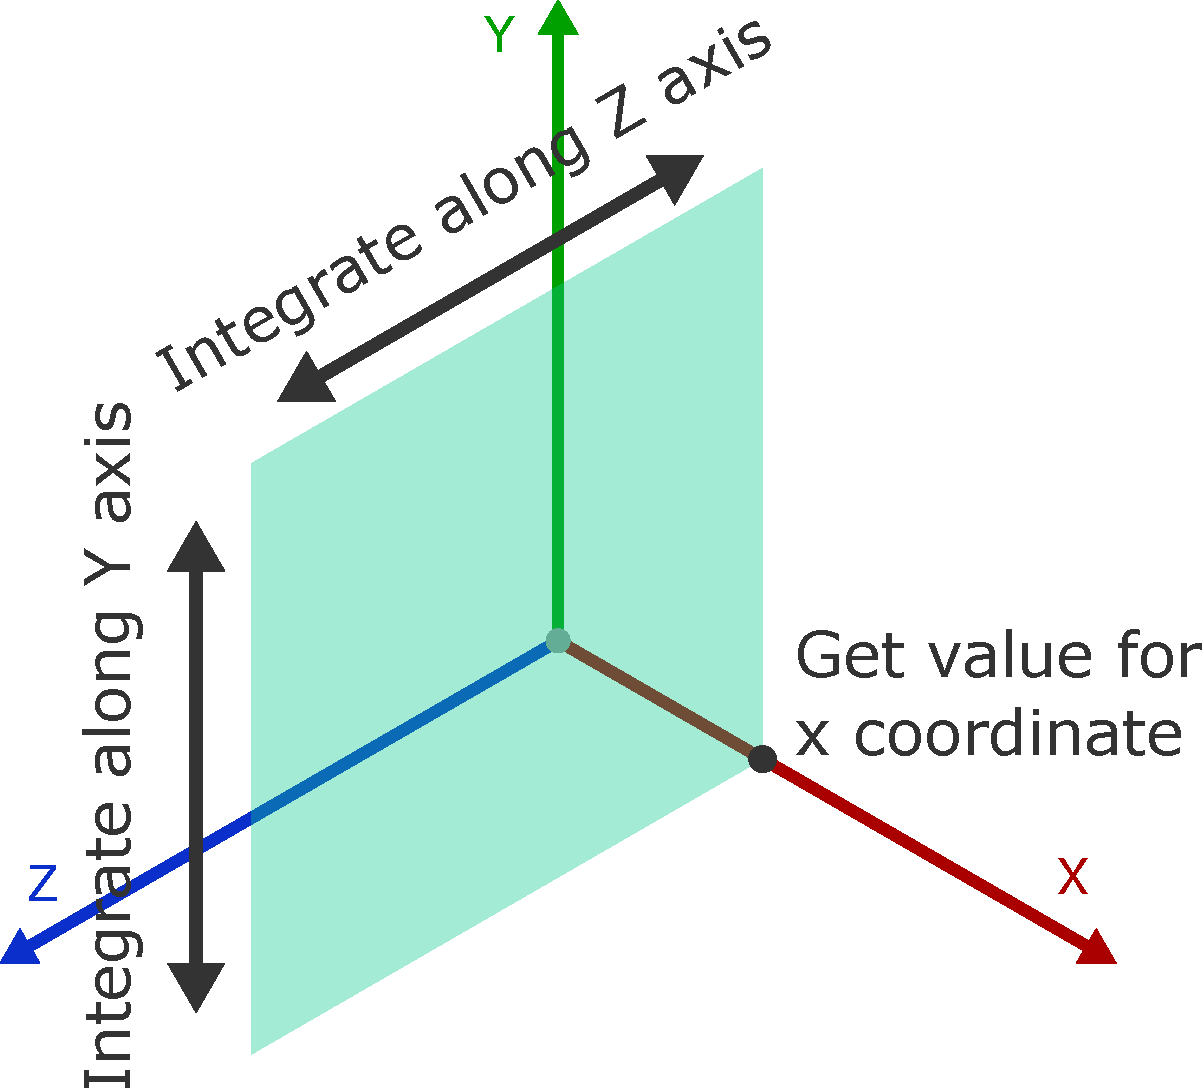
\includegraphics[width=0.5\textwidth]{figures/per_axis_plot_explained.pdf}
	\caption{Calculation method of the \textit{Per axis probability density} for a given $x$ coordinate}
	\label{fig:per_axis_explained}
\end{figure}
To obtain the plot of $\rho_X(x, t)$ per axis probability density we integrate the $\rho(\vec{r}, t)$ where $r_x = x$ and the other two coordinates run across their domain.
Equation \ref{eq:per_axis_calculation} gives the formula for calculating this measurable for the $X$ axis.
\begin{equation}
	\rho_X(x, t) = \int_Y \int_Z \rho(\vec{r}, t)\; dy dz
	\label{eq:per_axis_calculation}
\end{equation}
Figure \ref{fig:per_axis_explained} attempts to provide further intuition.
We also overlap the plot of the potential barriers on the same graph to understand the changes in propagation of the wave packet caused by the localized potential.
This type of plot can provide useful information for most of the simulation cases, but it is especially useful when we want to simulate the behavior of three one dimensional particles in a three dimensional configuration space.
In this case the projected probability density along each axis represents the wave packet of a different 1D particle.
It is possible to initialize a potential that models the collision between these three particles.
This creates the effect that the particles interact.
In the configuration file there is a possibility to set whether a potential barrier should appear in the visualization.
By disabling the visualization of the interaction potential we can get rid of any hardly conceptualizable elements of the resulting potential and maybe focus on a wall or a harmonic oscillator instead.
Probability density 3D is the most self explanatory output of the system.
Here we take the probability density as a 3D volumetric data set and visualize it using ray tracing.
Ray tracing is the method where we conceptually shoot rays of light from the virtual camera through the visualized volume.
Figure \ref{fig:ray_tracing_method} explains the concept of ray tracing.
\begin{figure}
	\centering
	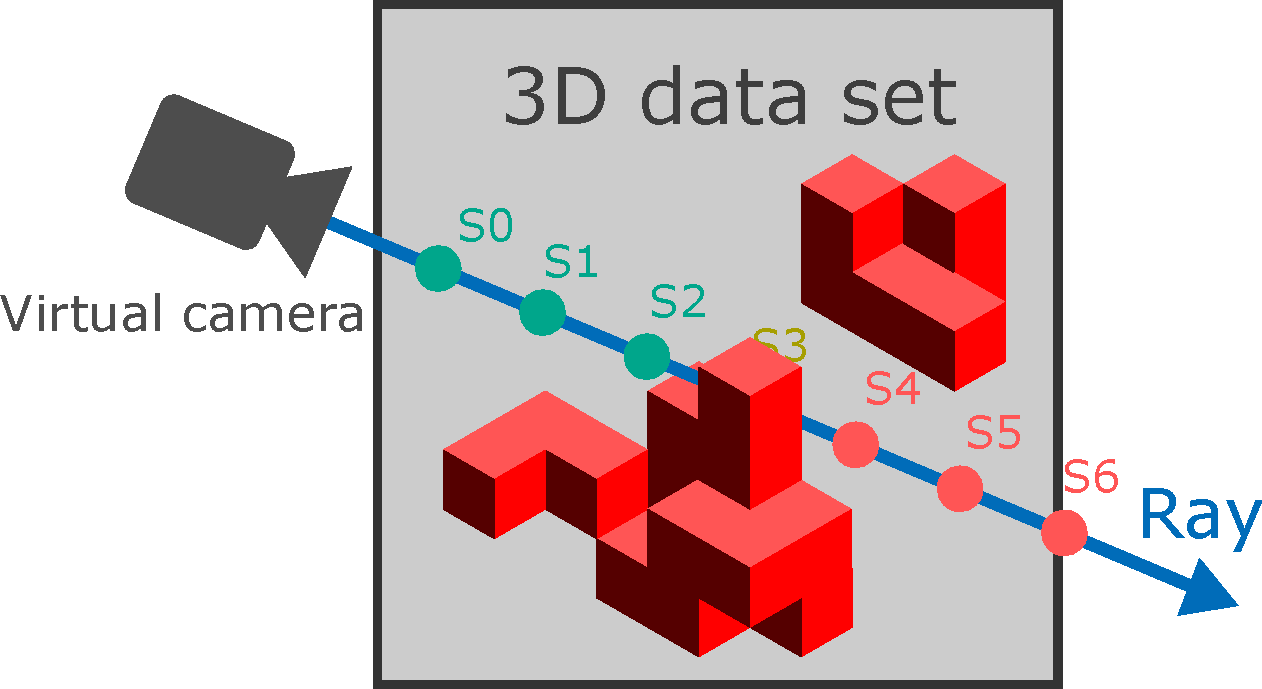
\includegraphics[width=0.75\textwidth]{figures/ray_tracing_visualization.pdf}
	\caption{Visual explanation of the ray tracing method: we sample the 3D data set along rays shot from the virtual camera}
	\label{fig:ray_tracing_method}
\end{figure}
For each pixel of the image there is exactly one ray.
We progress along the ray in discrete steps and at each step we sample the data set.
The data read from the volume has usually a single intensity value.
We interpret the data using a transfer function that determines the color and opacity that should be associated with the intensity.
The color and opacity is then combined along the ray resulting in the final color and opacity value for the pixel of the image.
The operator that recursively combines the color and opacity values is called under operator. For recursive calculation of the $A_n$ opacity in $n$th step along the ray it can be written in the form of
\begin{equation}
	\label{eq:under_op}
	A_n = A_{n-1} + \alpha_n(1 - A_{n-1})
\end{equation}
where $A_{n-1}$ is the opacity calculated at the previous step and $\alpha_n$ is the local opacity at the $n$th step.
A similar equation could be written for red, green and blue (RGB) color channels.
If we would only use the colors obtained by simply stepping through the sample points the look of the probability density would be rather dull.
We also utilize approximated gradient vectors.
One can calculate these vectors by taking the central difference using six additional samples around the currently sampled point.
(We however deployed a better method described later.)
The gradient vector points towards in the direction in which the probability density increases the fastest.
If we make the analogy that a solid body objects has also got gradient vectors right on the edge of it's surface so that these vectors point towards the inside of the object perpendicular to the surface
we can make the connection between gradient vectors and surface normals.
Normal vectors of a surface are unit length vectors pointing towards the outside world from the surface and are also perpendicular to the surface.
Normal vectors can be expressed as negated and normalized gradients.
Normal vectors are often used in various surface shading models, since they give a good description how surfaces reflect light.
Even tho our probability density has a much less clearly defined gradient this technique can still be used to obtain an approximated normal vector.
If this vector is sufficiently defined (the magnitude of the gradient is not too close to zero) than we can use simple shading model such as the Blinn-Phong reflection model \cite{Blinn1977} to enhance our visuals.
We even use the length information of the gradient to fade between the shaded and unshaded look.
We would like to mention that in our previous works we have experimented with more physically plausible shading techniques such as applying the Cook-Torrance \acrfull{brdf} \cite{CookTorrance1982}.
This however has not yielded good results for volumetric visualization since surface imperfections are calculated into the model thus the generally fussy nature of volumetric datasets result in an overall dark look.
The simple Blinn-Phong model however is cheap to compute, and provides sufficiently strong specular highlights while it's still easy to parameterize.
For most of our simulations we use a total simulated volume of $512\times 512 \times 512$ data points.
We leave the outer half of the total volume to accommodate the draining potential described in the last part of section \ref{sec:used_method}.
This means that so far we only visualize $50\%$ of the stored data set: $256 \times 256 \times 256$.
In the future we may experiment with reducing the space used up by the draining potential.
Until than we rely heavily on good reconstruction filters to get rid of the aliasing effects visible by sampling the data set of relatively low resolution.
We utilize Balázs Csébfalvi's reconstruction filter \cite{csebfalvi2023}.
This method provides consistent gradient estimation that is the analytic gradient of the reconstructed function.
It has an approximation order of three and it's also $C^1$ continuous.
This method evaluates eight trilinear samples to calculate the intensity and the gradient for a given point.
In current generation of \acrshort{gpu}s trilinear filtering can be efficiently evaluated using the built in sampling routines.
The eight is only one more sample compared to the seven used in the less advanced intensity plus central difference technique and we also get better result as shown in the referred paper.

The last type of the five different image outputs of our program we call \textit{Probability evolution}.
To create this output we divided the visible region of the simulated volume to separate partitions.
On these images of this type we display a plot where we integrate the probability density over these regions following equation \ref{eq:probability_evolution}.
\begin{equation}
	\probP(t)=\int_\mathcal{V}\rho(\vec{r},t)d^3r
	\label{eq:probability_evolution}
\end{equation}
Conceptually this gives us the probability of the event of the particle being found in these spatial regions.
It is also allowed to specify overlapping regions.
By doing so we only get the probability of non excluding events.
We prefer to create a measurement region for the entirety of the visible volume.
This is very informative when the particle leaves the visible parts, hence the probability of the particle being found somewhere inside the visible part drops below one.
Note that modeling such scenarios is made possible by using the draining potential.

Besides the sequence of images our program also renders two animations in MP4 format.
One is created from a sequence of images rendered as in the \textit{Probability density 3D} sequence.
The other is the animated version of the \textit{Per axis probability density} sequence.
The rate at which the state of the simulation is captured as an animation frame and the playback frame rate can be configured separately.

\subsection{Performance test}

We measured the performance of our application.
We used a personal laptop to run and test the program.
The system specification of our computer is summarized in figure \ref{fig:system_spec}.
\begin{figure}
	\begin{center}
		\begin{tabular}{|m{5em}||m{25em}|}
			\hline
			CPU & AMD Ryzen 5 6600H with Radeon Graphics            3.30 GHz\\
			\hline
			GPU & NVIDIA GeForce RTX 3050 Ti Laptop GPU\\		
			\hline
			RAM & 16 GB\\		
			\hline
			OS & MS Windows 11 64-bit\\		
			\hline
		\end{tabular}
		\caption{System specification of the used test hardware}
		\label{fig:system_spec}
	\end{center}
\end{figure}
First we tried a \acrshort{cpu}-only version of our simulator to compare the results with the \acrshort{gpu} accelerated implementation.
The results of the comparison can be found in figure \ref{fig:performance_test}.
\begin{figure}
	\begin{center}
	\begin{tabular}{|m{8em}||m{8em}| m{8em}| m{4em}|}
		\hline
		Input size & CPU-only Avg. [iter/s] & GPU~accelerated Avg. [iter/s] & Avg. speed up\\
		\hline
		$128 \times 128 \times 128$ & $1.1$ & $11.5$ & $\times 10.45$\\
		\hline
		$256 \times 256 \times 256$ & $0.09$ & $6.5$ & $\times 72.22$\\
		\hline
		$512 \times 512 \times 512$ & $0.01$ & $0.5$ & $\times 50.00$\\
		\hline
	\end{tabular}
	\caption{Results of a performance test using a CPU-only and a GPU accelerated version of the application averaged}
	\label{fig:performance_test}
\end{center}
\end{figure}
Here we tested three different configurations with varying resolution.
We measured the average iteration count per second.
The test shows that by using \acrshort{gpu} acceleration we obtained significant speed up over the the \acrshort{cpu}-only implementation.








	\section{Results}
\label{sec:results}

\subsection{General approach and used unit system}

We used our software to perform various \acrshort{wpd} simulations.
In this section, we present the results of some of these simulations.
We will shortly introduce the simulated scenarios.
We also want to provide some formulas to validate the correctness of some of the simpler scenarios analytically.
Our simulator uses the Hartree atomic units \cite{hartree_1928}.
Every quantity in the upcoming part should be interpreted as such.
This unit system makes it convenient to deal with quantities at atomic scale.
You can find animations showing the time evolution of \acrshort{wp}s simulated by our software on  \url{https://zoltansimon.info/src/content/research/wavepacketsim.html}.

\subsection{Double-slit experiment}

First, we would like to present the simulation results of an electron scattering experiment.
Scattering of a particle happens when the \acrshort{wp} of the particle passes through some kind of a barrier with holes in it.
In our simulation, we can model the barrier as a specifically initialized localized potential.
The \acrshort{wp} arrives from one side of the barrier.
While passing through this barrier, it scatters, and some of the \acrshort{wp} gets reflected back.
The portion of the \acrshort{wp} that passed through --suffering scattering-- continues forward and consequently arrives at a measuring device\footnote{In scattering and diffraction experiments we can make the distinction between a near field and far field solution.}.
In our simulation, our measuring device is a virtual canvas where we measure the probability density.
A simple scattering scenario is the double-slit experiment.
Here the barrier is a potential wall with two narrow parallel slits.
The \acrshort{wp} passes through these slits.
According to the Huygens–Fresnel principle in scattering experiments, we can approximate the wave function after the barrier as concentric waves emitted from the slits or holes of the barrier.
This gives a simple enough model to predict the shape of the interference pattern forming on the canvas.
We would like to validate the distance between the stripes in the interference pattern.
To calculate the distance between the probability density peaks, first, we have to get a formula for the intensity on the canvas.
\begin{equation}
	\label{eq:Huygens}
	I(\vec{r}) = I_0 \frac{sin^2\left( \pi N \frac{dy}{\lambda L} \right)}{sin^2\left( \pi \frac{dy}{\lambda L} \right)}
\end{equation}
where $N$ is the number of holes on the barrier (in double-slit experiment $2$), $d$ is the distance between the center of the holes, $L$ is the distance between the canvas and the barrier $\lambda$ is the wavelength of the wave and $y$ is the location on the canvas.
We performed the simulation using $L = 30$ Bohr radii, $d = 4.0$ Bohr radii, $\lambda = \frac{2\pi}{3}\simeq 2.1$ Bohr radii with two slits.
The width of each slit was a small enough value of $1.0$ Bohr radii.
\begin{figure}
	\begin{center}
		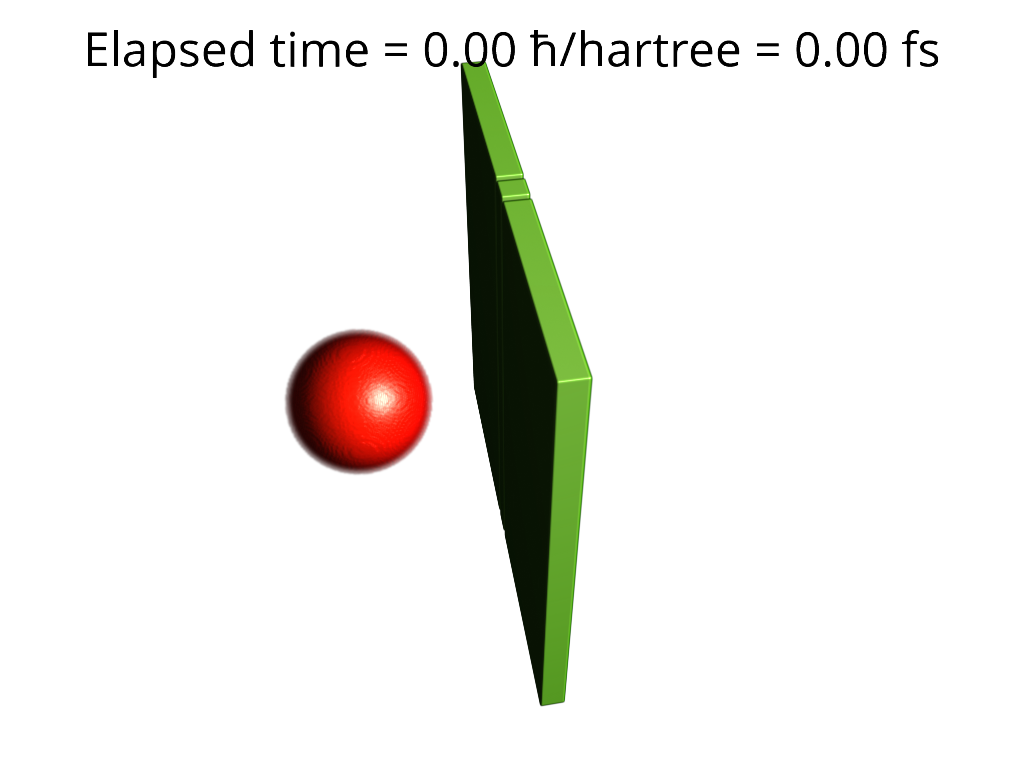
\includegraphics[width=0.5\textwidth]{figures/double_slit_01.png}
		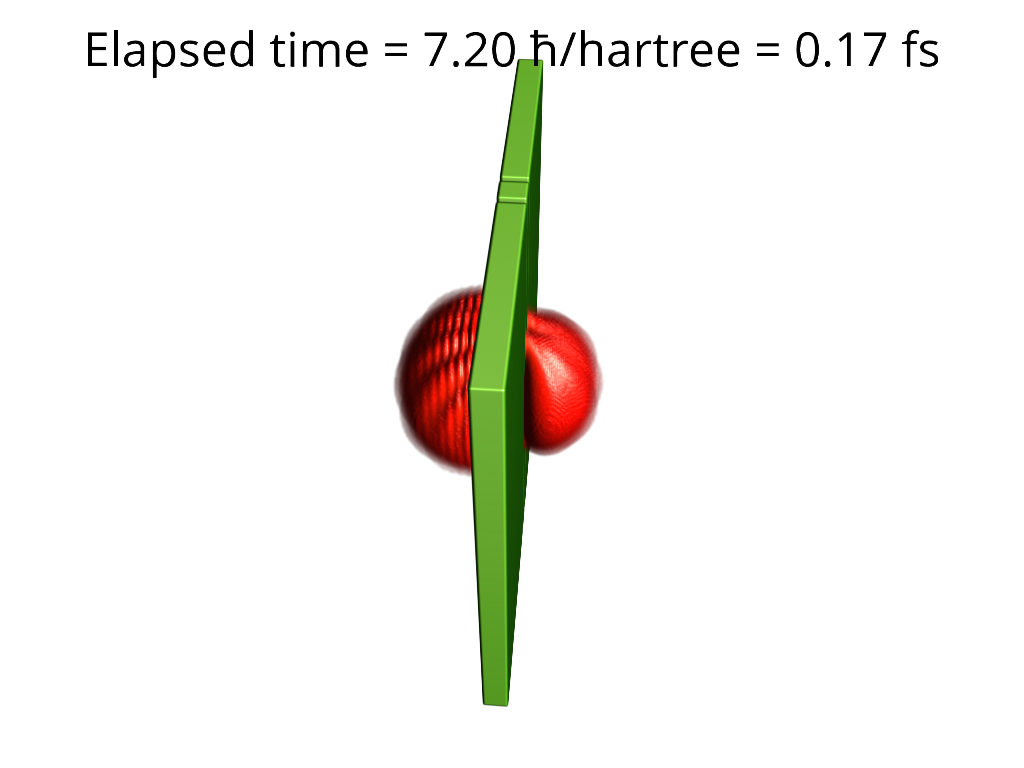
\includegraphics[width=0.5\textwidth]{figures/double_slit_02.png}
		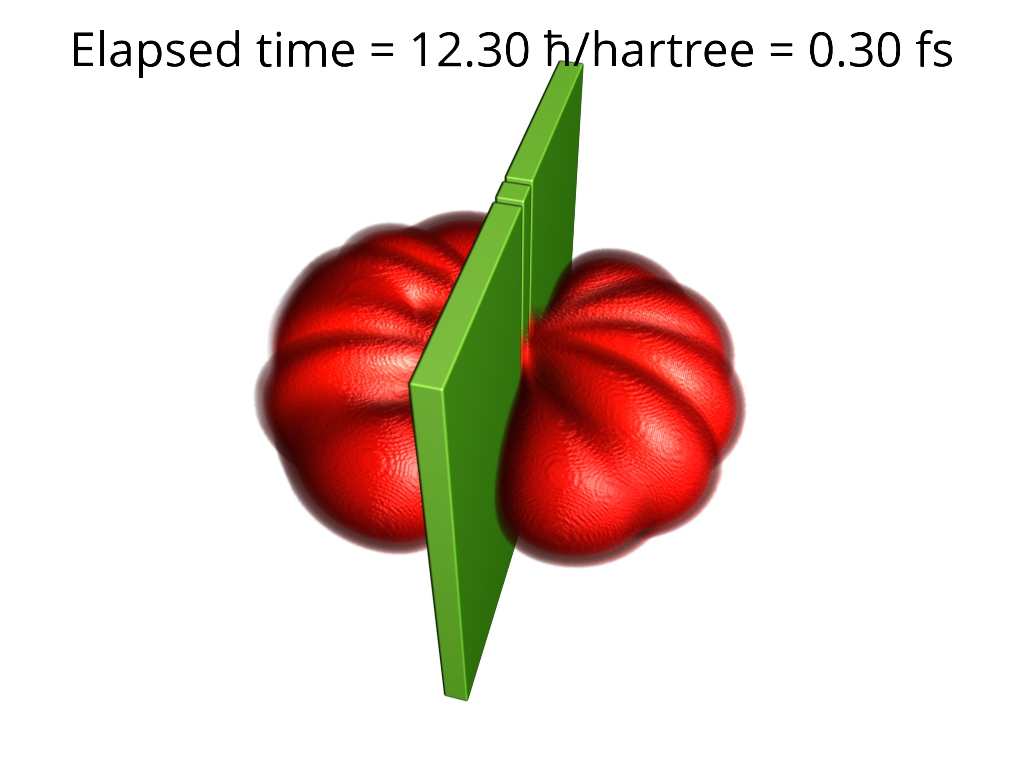
\includegraphics[width=0.5\textwidth]{figures/double_slit_03.png}
		\caption{Stages of the double-slit experiment: before, during, and after passing through the double-slit}
		\label{fig:double_slit_stages}
	\end{center}
\end{figure}
Different stages of double-slit simulation can be seen in figure \ref{fig:double_slit_stages}, where we have used ray tracing to visualize the probability density and the potential.
The interference pattern is visualized in figure \ref{fig:double_slit_interference} on a canvas of size $60 \times 60$ Bohr radius.
We compared the simulated pattern and the pattern predicted by the Huygens–Fresnel principle.
It can be seen that the two patterns are very similar.
The animation of this simulation can be accessed on \url{https://www.youtube.com/watch?v=16M21MPFea0}.
\begin{figure}
	\begin{center}
		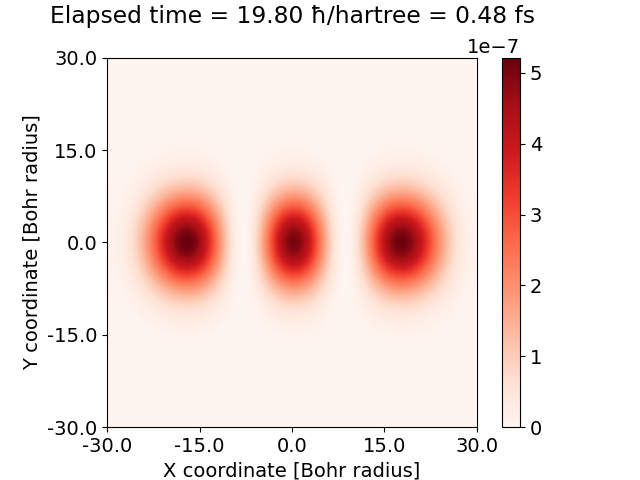
\includegraphics[width=0.6\textwidth]{figures/double_slit_interference.png}
		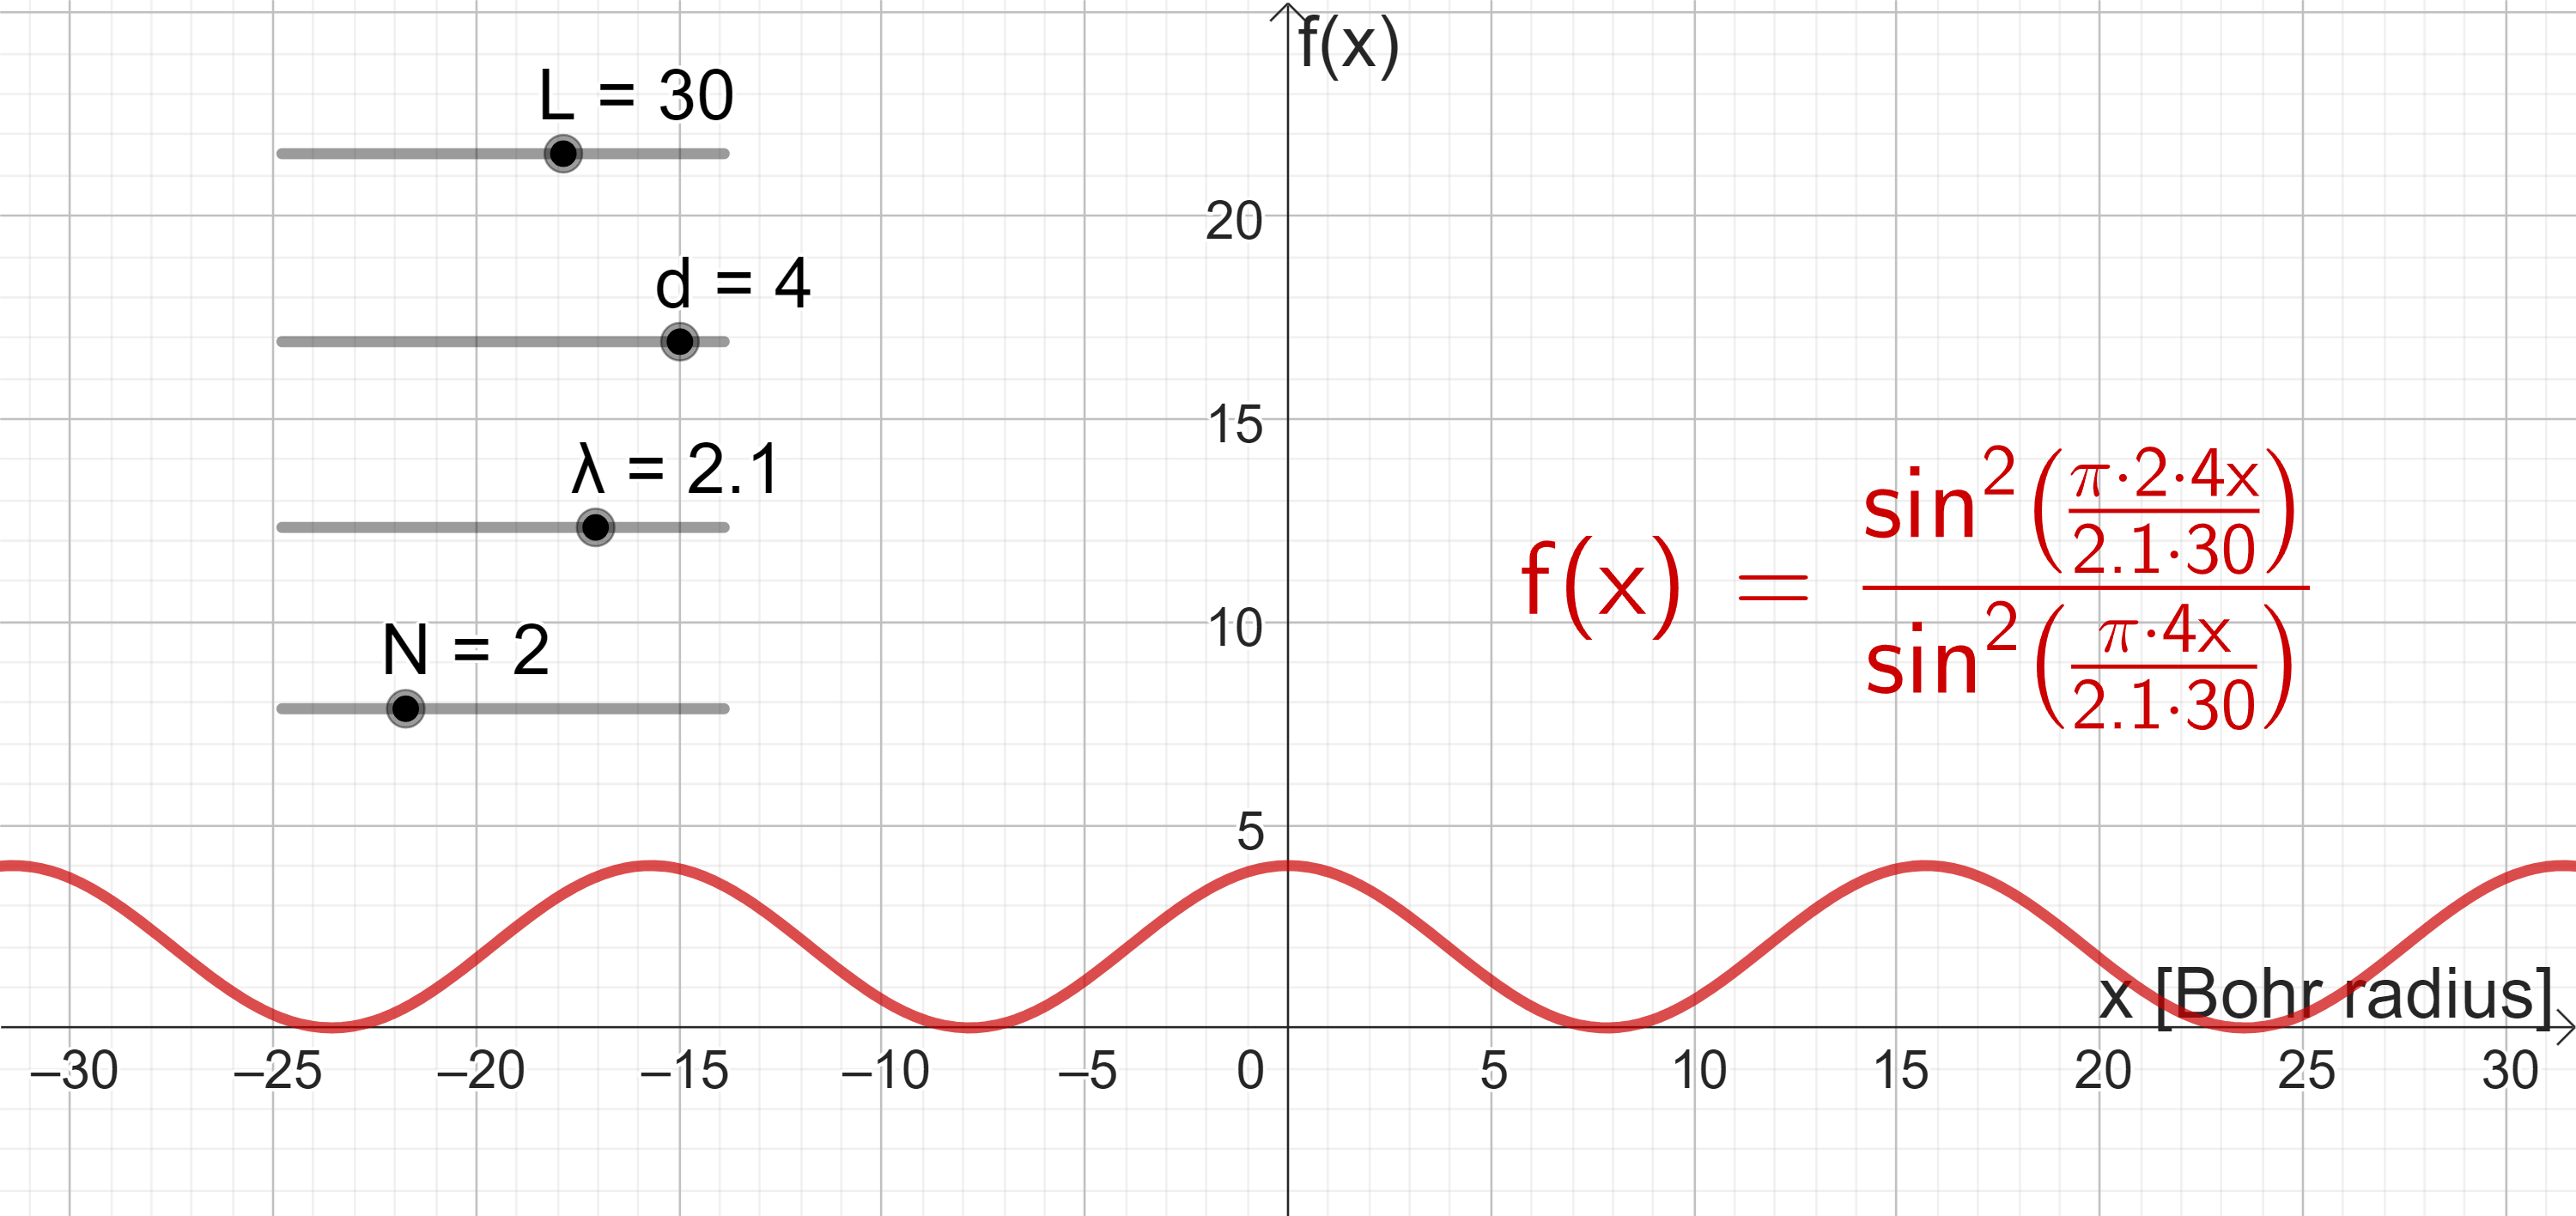
\includegraphics[width=0.6\textwidth]{figures/validation_of_double_slit.png}
		\caption{Comparison of the simulated (above) and the analytically predicted (below) interference pattern during double-slit experiment}
		\label{fig:double_slit_interference}
	\end{center}
\end{figure}

\subsection{Diffraction by optical grating-like potential}

Many different forms of diffraction can be explained using \acrshort{qm}.
The scale at which diffraction happens ranges from the scale of subatomic particles to larger molecules.
Measuring diffraction patterns is a handy tool in the hands of scientists.
It provides information about the object that caused the diffraction.
At this point, it is essential to emphasize that the diffraction of light is a different phenomenon from the diffraction of matter waves since light is an electromagnetic wave.
With that said, the fact that particles are not electromagnetic waves but still exhibit wave-like behavior, as discussed in Section \ref{sec:theory} makes this experiment even more interesting.
Note that in equation \ref{eq:Huygens}, the $y$ is a one-dimensional coordinate. Indeed, the double-slit experiment can be fully described using only two spatial dimensions, and the diffraction pattern forms in a single dimension perpendicular to the propagation direction of the wave.
This is because the localized potential in this scenario is independent of the $z$ coordinate.
To make use of all three simulated dimensions, we also modeled diffraction on diffraction gratings.
In optics, a diffraction grating is a periodic 2D structure that diffracts light \cite{Stroke1967}.
In \acrshort{qm}, such gratings can also be utilized to diffract wave packets.
The holes between the potential nodes behave like the holes in the double-slit experiment.
We put 11 nodes in each direction, forming a rectangular grid.
We experimented with various lattice constants (distance between adjacent grid points).
Here, we present two simulations.
In the first simulation, each node has a Gaussian potential distribution and a maximal potential of $V_{max} = 8$ hartree.
The distance between adjacent grid points is $d = 4$ Bohr radii.
In the second simulation, each node has a Gaussian potential distribution and a maximal potential of $V_{max} = 25$ hartree.
The distance between adjacent grid points is $d = 8$ Bohr radii.
The canvas distance is $L=30$ Bohr radii, and the wavelength of the \acrshort{wp} is $\lambda\simeq 2.1$ Bohr radii for both simulations.
Note in both cases the kinetic energy of the \acrshort{wp} $E = \frac{p^2}{2m} = \frac{h^2}{2\lambda^2} \simeq 4.5$ hartree is less than $V_{max}$.
Otherwise, the grating would not impact the propagation of the \acrshort{wp} sufficiently.
In figure \ref{fig:optical_grid_stages}, we visualized different stages of the time development of the first simulation, and \ref{fig:optical_grid_stages_8_bohr_radii} showcases stages of the second simulation.
Both sequences of rendered images make use of the ray tracing visualization method.
\begin{figure}
	\begin{center}
		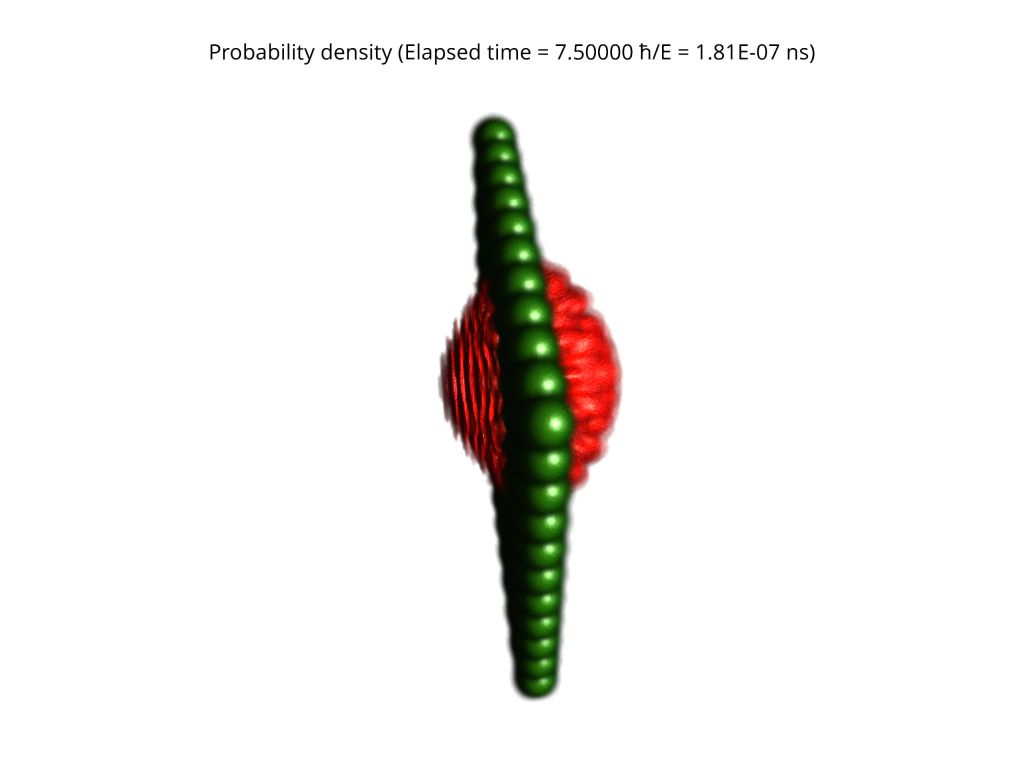
\includegraphics[width=0.5\textwidth]{figures/optical_grid_01.png}
		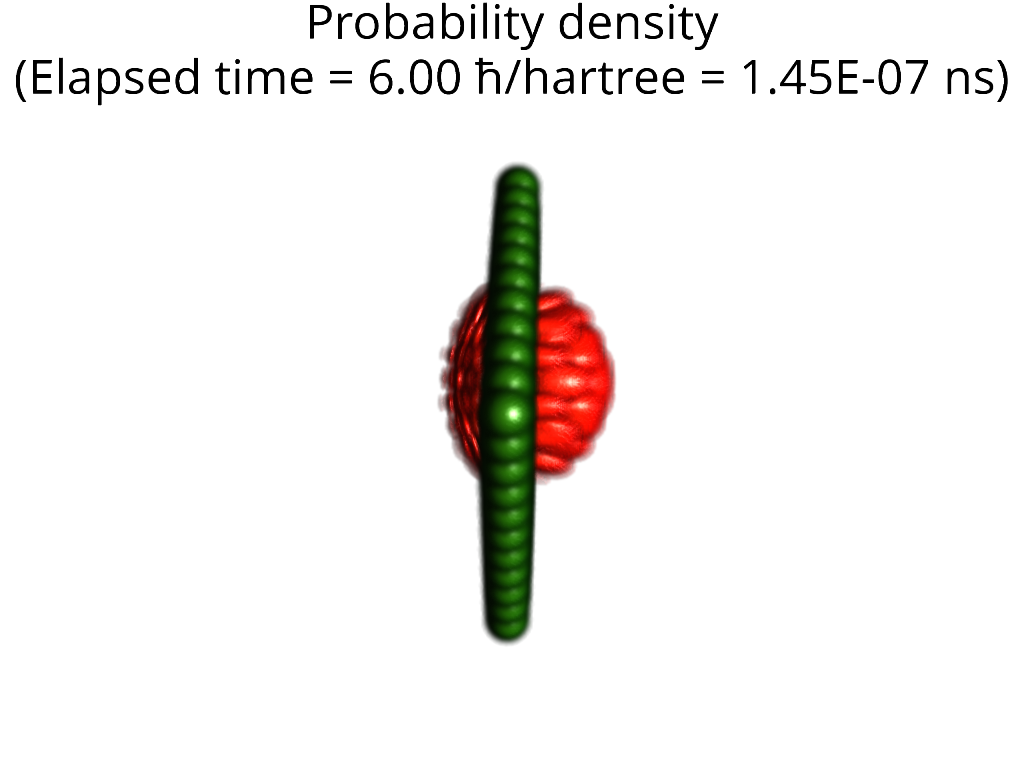
\includegraphics[width=0.5\textwidth]{figures/optical_grid_02.png}
		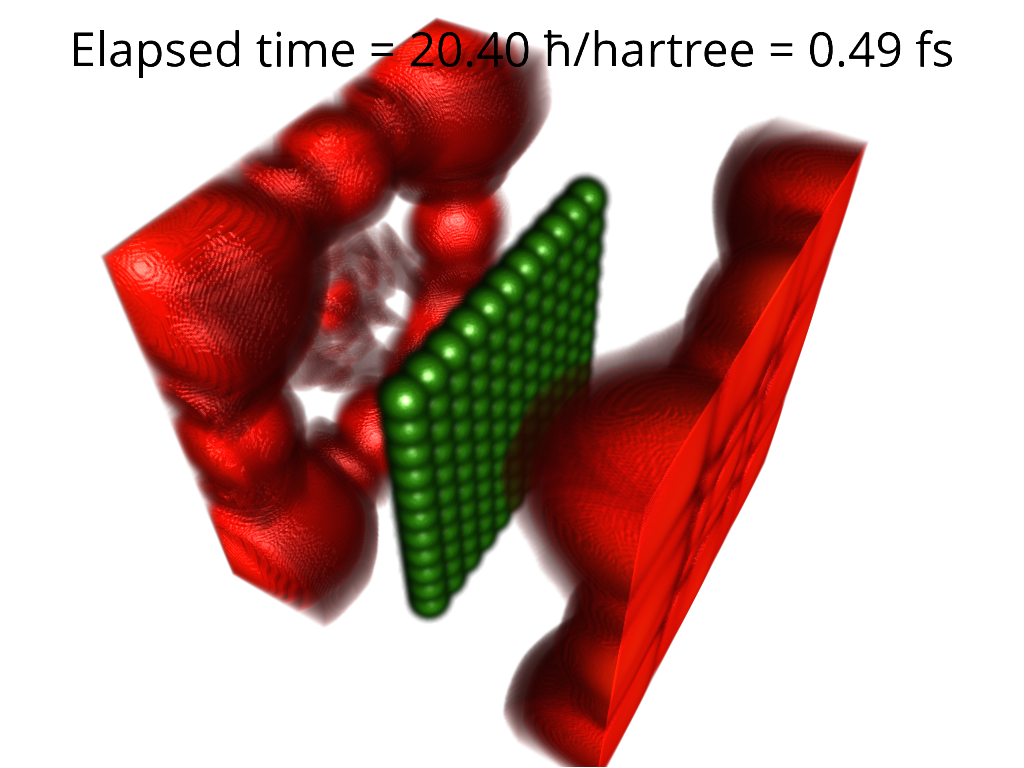
\includegraphics[width=0.5\textwidth]{figures/optical_grid_03.png}
		\caption{Stages of the optical grid experiment using a grid with lattice constants of $4$ Bohr radii: during, right after, and later after passing through the grid}
		\label{fig:optical_grid_stages}
	\end{center}	
\end{figure}
\begin{figure}
	\begin{center}
		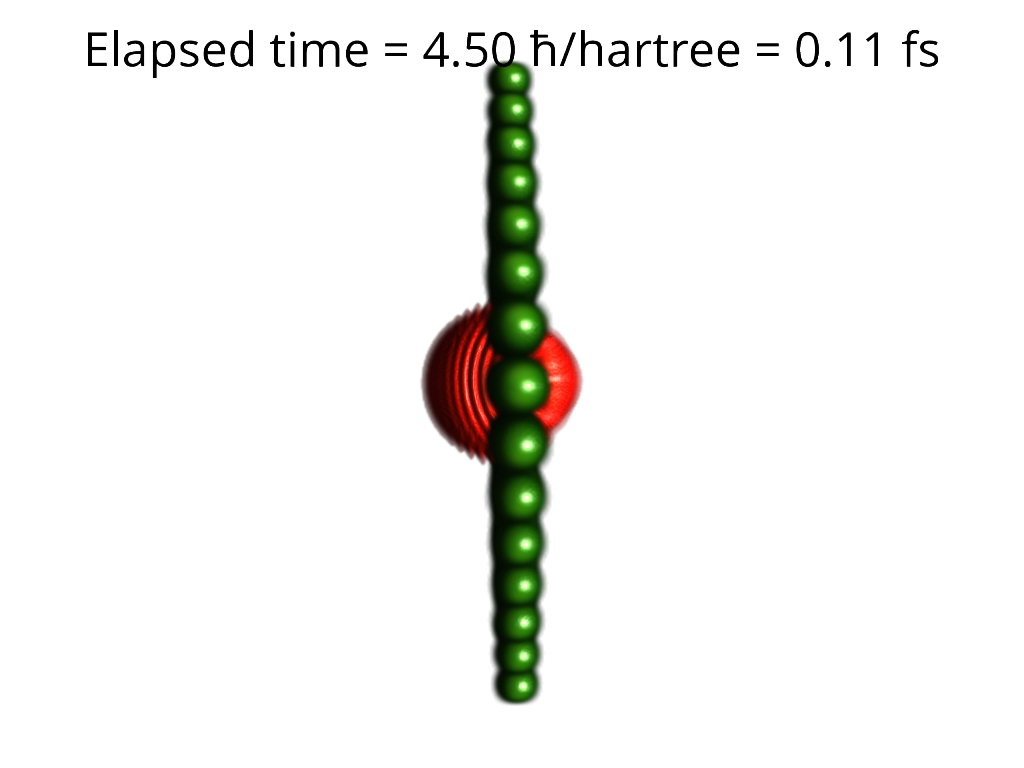
\includegraphics[width=0.5\textwidth]{figures/optical_grid_8_bohr_rad_01.png}
		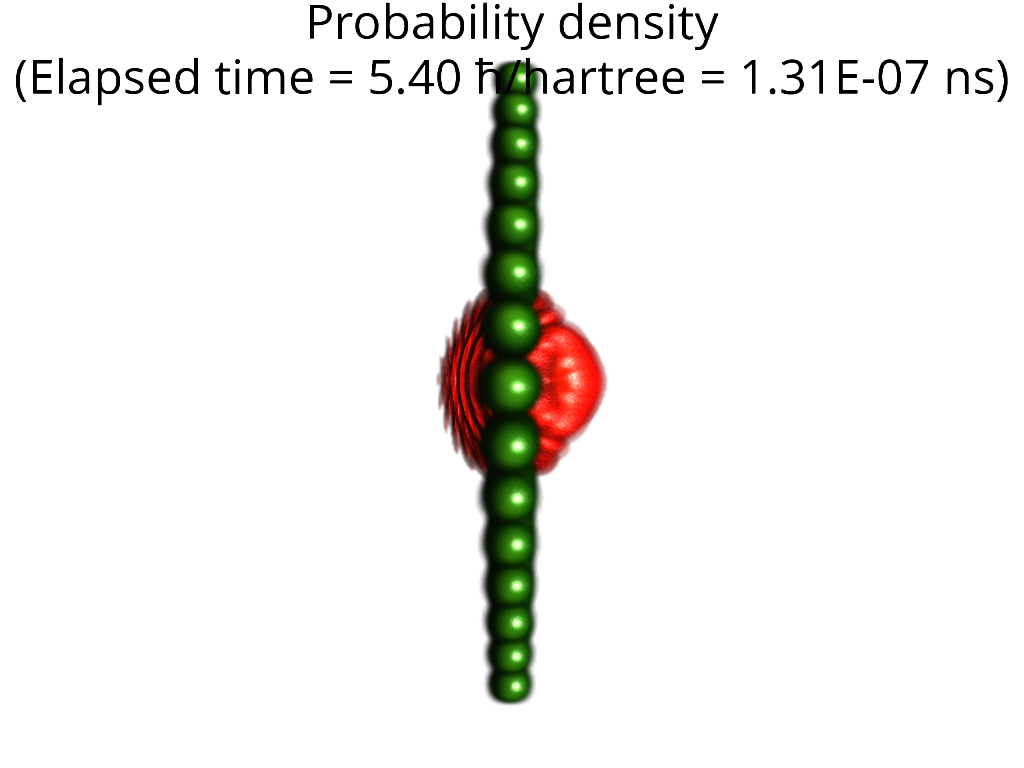
\includegraphics[width=0.5\textwidth]{figures/optical_grid_8_bohr_rad_02.png}
		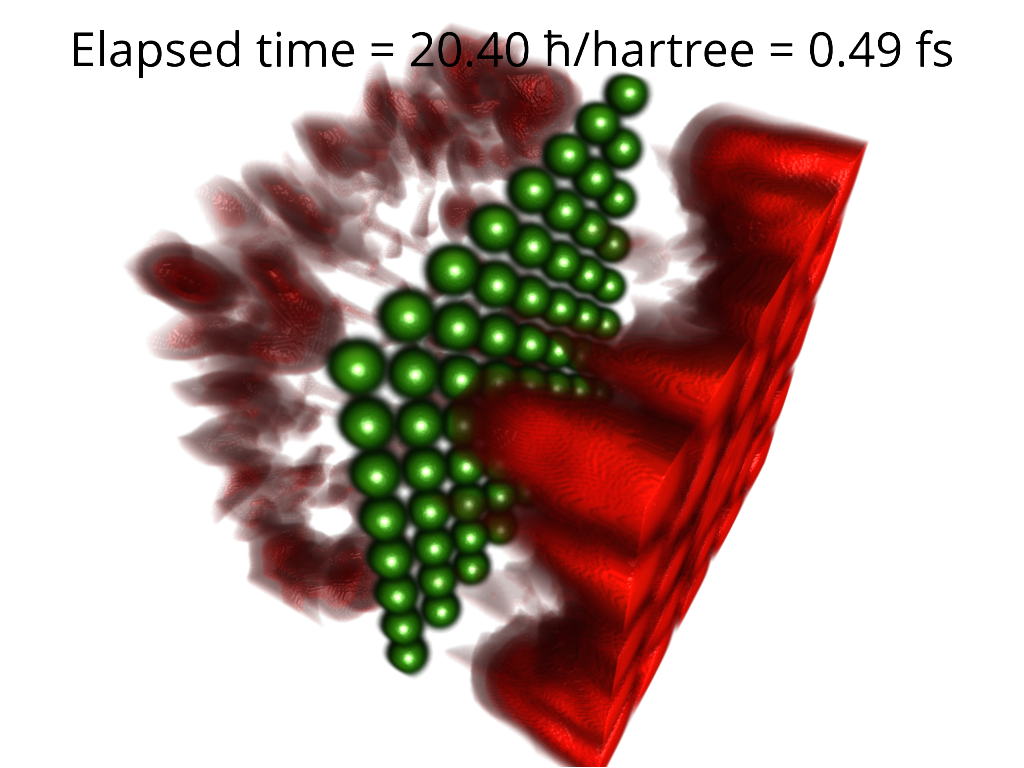
\includegraphics[width=0.5\textwidth]{figures/optical_grid_8_bohr_rad_03.png}
		\caption{Stages of the optical grid experiment using a grid with lattice constants of $8$ Bohr radii: during, right after, and later after passing through the grid}
		\label{fig:optical_grid_stages_8_bohr_radii}
	\end{center}	
\end{figure}

During the simulation, many interesting interference patterns arise.
We showcase some of these for the $4$ Bohr radius lattice constant case in figure \ref{fig:optical_grid_interference} and for the $8$ Bohr radius lattice constant case in figure \ref{fig:optical_grid_interference_8_grid}.
The animations showing the results in motion can be found on \url{https://youtu.be/KCE5xqm-diQ?si=-kzjWvaw8zOcAz4C} and \url{https://youtu.be/YCadOpsx9y8}.
\begin{figure}
	\begin{center}
		
\includegraphics[width=0.49\textwidth]{figures/optical_grid_interference_01.png}
		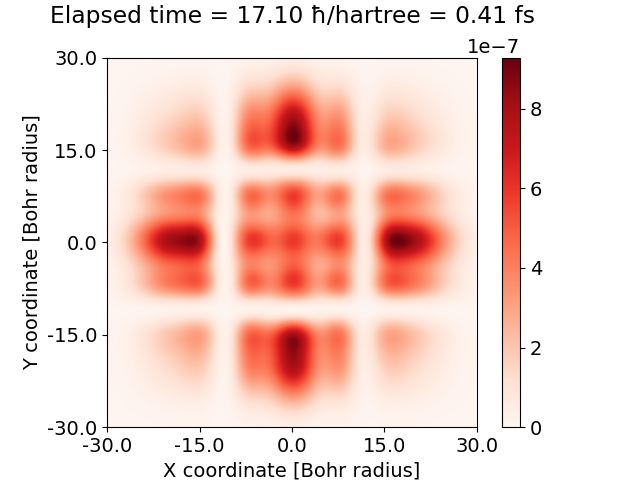
\includegraphics[width=0.49\textwidth]{figures/optical_grid_interference_02.png}
		\caption{Two stages of interference patterns forming on the measurement canvas during optical grid simulation using lattice constant of $4$ Bohr radii}
		\label{fig:optical_grid_interference}
	\end{center}	
\end{figure}
\begin{figure}
	\begin{center}
		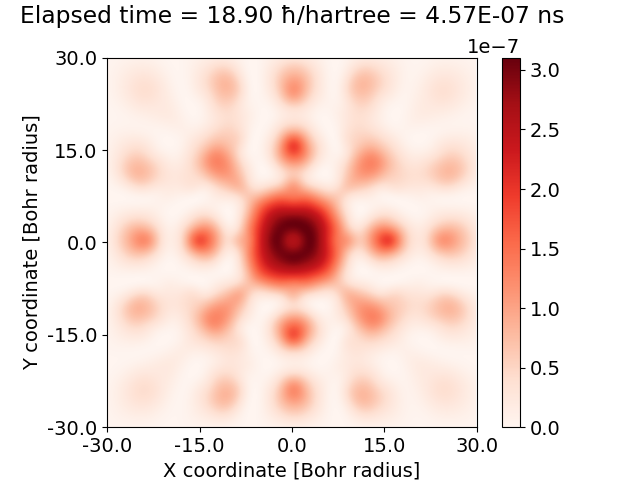
\includegraphics[width=0.49\textwidth]{figures/optical_grid_interference_01_8_grid.png}
		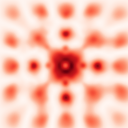
\includegraphics[width=0.49\textwidth]{figures/optical_grid_interference_02_8_grid.png}
		\caption{Two stages of interference patterns forming on the measurement canvas during optical grid simulation using lattice constant of $8$ Bohr radii}
		\label{fig:optical_grid_interference_8_grid}
	\end{center}	
\end{figure}

\subsection{Simulating 1D particles in 3D configuration space}

One interesting use case of a higher dimensional \acrshort{wpd} simulator is that the higher dimensional space can be used to model the interactions between multiple lower-dimensional particles.
For example, our 3D simulation is capable of the simulation of three 1D particles.
To do this, we have to define special interaction potential.
To create such potential, we have to think about the coordinates in the higher dimensional configuration space as the coordinates of the lower dimensional space describing the location of the lower dimensional particle.
If the potential energy affecting all particles can be expressed as a $V(x_a, x_b, x_c)$ function of the location of particle $A$ and $B$ and $C$, then we can reinterpret this function as the $V(\vec{r})$ localized potential function used in the potential propagator in equation \ref{eq:potential_prop}.
Note that here $\vec{r}$ becomes $(x_a, x_b, x_c)$.
To model the interaction between the three 1D particles, we initialized a linear combination of two types of interaction potentials.
One is proportional to $\frac{1}{|x_i - x_j|}$ where $i,j\in\{a,b,c\}$ and $i\neq j$ and the other is a hard interaction that takes its maximum if the particles approach each other inside an $\epsilon$ radius otherwise it is zero.
To prevent blotting of the Gaussian \acrshort{wp} we also initialized a harmonic oscillator potential.
This helps because the Gaussian \acrshort{wp} is the eigenstate of the harmonic oscillator.
The potential for a harmonic oscillator is given in the following form
\begin{equation}
	\label{eq:harmonic_osc}
	V(x) = \frac{m\omega^2}{2}x^2
\end{equation}
where $m$ is the oscillating mass and $\omega$ is the angular frequency of the oscillation.
Our first simulation of 1D particles is somewhat similar to the classical Newton's cradle \cite{}
in the sense that it demonstrates momentum transfer between multiple particles.
We created a scenario where particle $A$ starts at $25$ Bohr radii away from the center of the oscillator where the potential energy is maximal; thus, it accelerates towards the other two particles ($B$ and $C$), consequently transferring the momentum to particle $C$ on the far right.
For this experiment, the interaction potential consists only of the hard interaction.
The angular frequency of the oscillator was selected to be $\omega = \frac{2\pi}{40} \simeq 0.1571\; \frac{rad\cdot hartree}{\hbar}$.
After the momentum transfer, particle $C$ propagates towards the maximal potential of the oscillator on the far right.
Particle $B$ stays in place since it serves only as a medium in the momentum transfer.
The momentum gained from particle $A$ was immediately given to particle $C$.
When all the kinetic energy of the moving particle is transferred to potential energy, then it turns back.
The oscillation with the momentum transfer between the particles continues.
Different phases of this simulation can be observed on the per-axis visualization in figure \ref{fig:1d_particles_in_oscillator_stages}.
The corresponding animation can be found on \url{https://youtu.be/zOiYACVOssU}.
\begin{figure}
	\begin{center}
		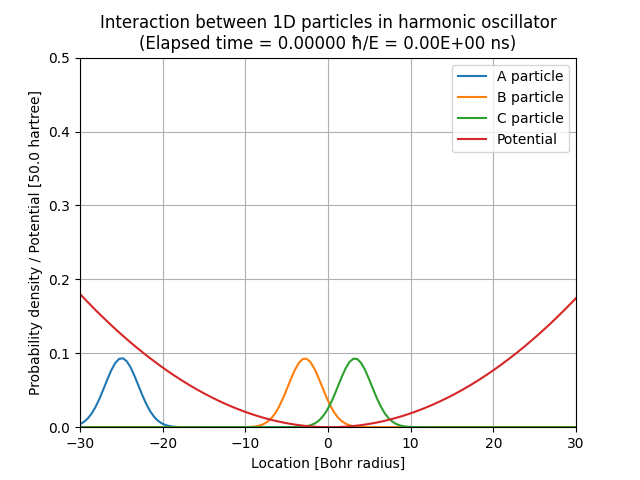
\includegraphics[width=0.6\textwidth]{figures/1d_oscillator_01.png}
		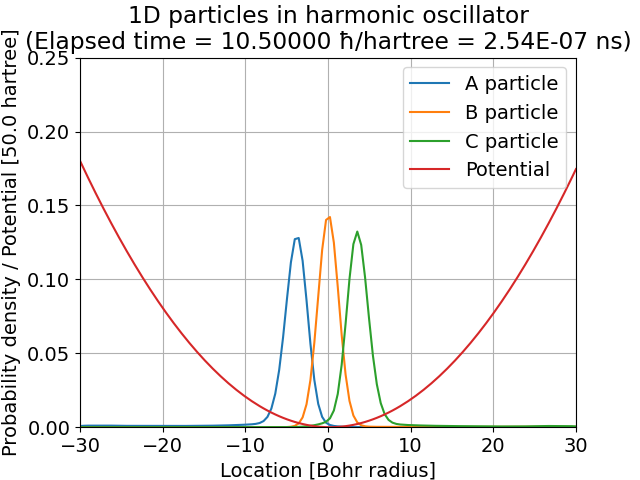
\includegraphics[width=0.6\textwidth]{figures/1d_oscillator_02.png}
		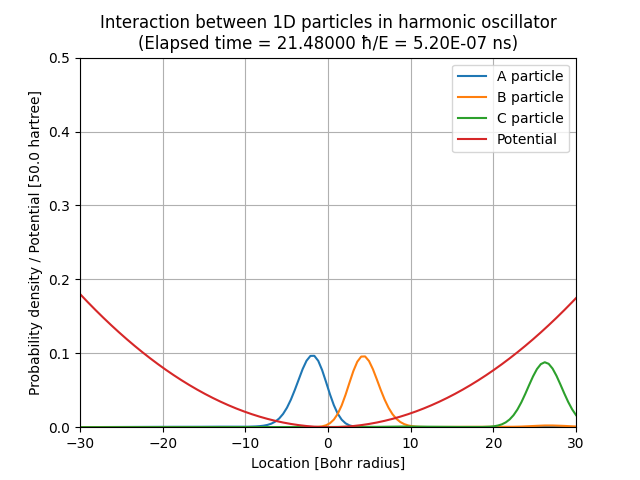
\includegraphics[width=0.6\textwidth]{figures/1d_oscillator_03.png}
		\caption{Stages of the interactions between 1D particles in harmonic oscillator: initial state, particle A giving momentum to particle C, particle C reaching maximal potential and turning back}
		\label{fig:1d_particles_in_oscillator_stages}
	\end{center}
\end{figure}
Please note that particle $C$ converts all of its kinetic energy to potential energy right at the half of the first period of the oscillation $t = 40 / 2 \frac{\hbar}{hartree} = 20 \frac{\hbar}{hartree}$.
This means that the harmonic oscillator functions correctly.

Now, let us repeat this experiment, but now we place a finite potential barrier in the middle of the oscillator.
In Tamás Geszti's book \cite{geszti2007}, we can find that the probability of a particle with $E$ energy tunneling through a $d$ thick barrier of $V_0$ potential can be expressed in the following form
\begin{equation}
	\label{eq:tunneling_probability}
	\probP_{tunnel} = \frac{1}{1 + \frac{V_0^2}{4E(V_0 - E)}sinh^2(\kappa d)}
\end{equation}
where $\kappa = \sqrt{2m(V_0 - E)}\;/\hbar$ is determined by the energy of the incoming \acrshort{wp}.
Energy is conserved, so $E = V(x_A)$.
We solve for $\probP_{tunnel} = \frac{1}{2}$.
One possible solution is $V_0 \simeq 9.8$ hartree and $d \simeq 0.3$ Bohr radius.
Particle $A$ gives its momentum to $B$ as before.
With these parameters, approximately half of the probability density of particle $B$ tunnels through the barrier, giving its momentum to particle $B$ on the next side of the wall.
This causes the $C$ to start moving with a probability of approximately $\frac{1}{2}$.
What we just described is called the entanglement of the states of particles $A$, $B$, and $C$.
Let's perform a measurement to determine the location of particles $A$, $B$, and $C$ shortly after the first momentum transfer could have happened.
If we would measure particle $A$ to be located in the middle of the harmonic oscillator, that means that it gave its momentum to particle $B$ and $B$ has tunneled through the finite potential barrier.
If $B$ tunneled, that also means that beyond the barrier, it collided with particle $C$, consequently transferring all its kinetic energy to $C$.
On the contrary, if the result of the measurement determining the location of particle $A$ would have shown that particle $A$ bounced back from $B$, that means that $B$ did not tunnel through the barrier.
This also means that particle $C$ did not receive any kinetic energy and stayed stationary right beyond the barrier.
The measurement of the state of one entangled particle determines the outcome of the measurement of the other entangled particles.
Real-life experiments are sound with this thought experiment \cite{Vasilyev2017}.
The probability density plot can be observed in figure \ref{fig:1d_osc_with_tunneling}.
The animation of this simulation can be found on \url{https://youtu.be/IVb_mpzmuYA}.
\begin{figure}
	\begin{center}
		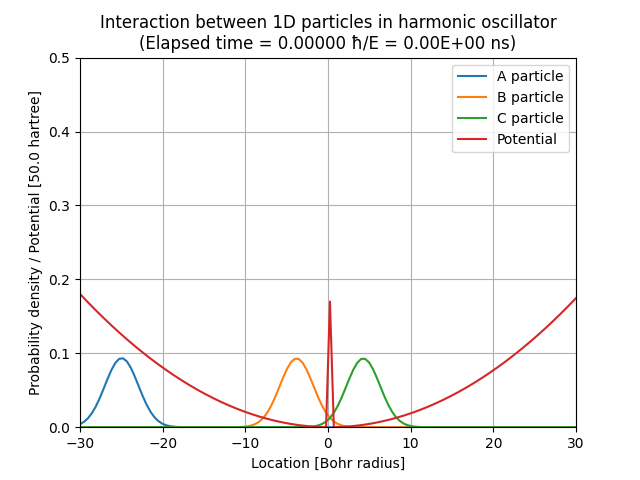
\includegraphics[width=0.6\textwidth]{figures/1d_oscillator_tunneling_01.png}
		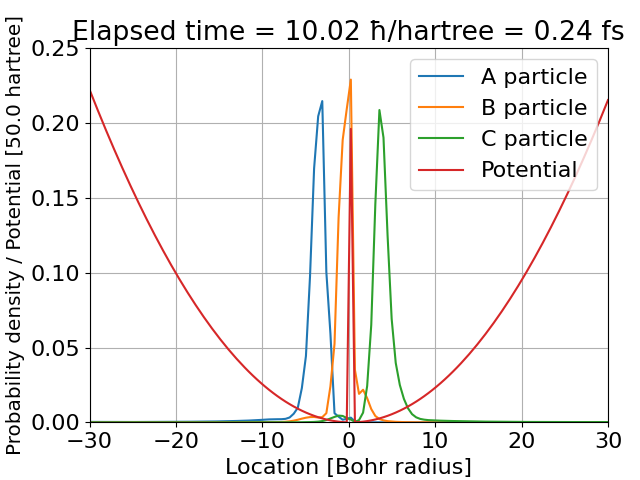
\includegraphics[width=0.6\textwidth]{figures/1d_oscillator_tunneling_02.png}
		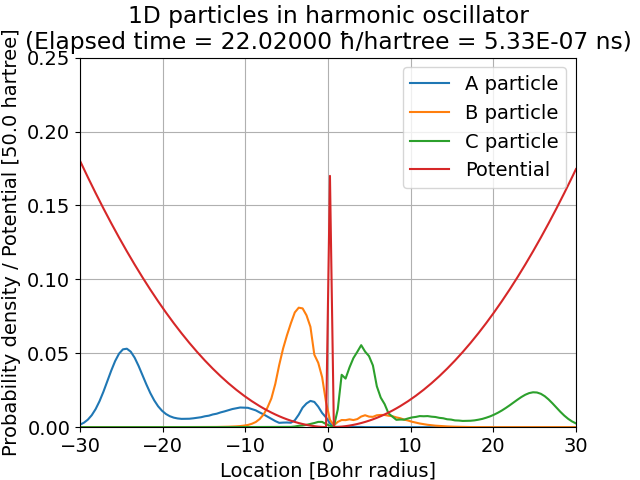
\includegraphics[width=0.6\textwidth]{figures/1d_oscillator_tunneling_03.png}
		\caption{Stages of the interactions between 1D particles in harmonic oscillator with finite potential barrier: initial state, particle A giving momentum to particle C with approximately 0.5 probability, particle C reaching maximal potential and turning back with approximately 0.5 probability}
		\label{fig:1d_osc_with_tunneling}
	\end{center}	
\end{figure}

\subsection{Modeling a flash memory cell}

Our last group of simulations tries to model the working of a flash memory cell.
Flash memory is used extensively in many modern electronic devices such as smartphones, laptops, or tablets.
The general structure of a cell is visualized in figure \ref{fig:flash_memory}.
The structure of a flash memory cell resembles a \acrfull{mosfet} \cite{Korec2011}.
The difference is that the memory cell has two gates: the control gate, which is connected to a control line similarly to regular transistors, and the floating gate, which is insulated from all sides by oxide layers.
Both the control gate and the floating gate are made out of conducting material (metal or polysilicon).
In figure \ref{fig:flash_memory}, it can be seen that between the control gate and the floating gate, there is a thicker potential barrier.
This prevents the flow of electrons between these two parts.
Only the Coulomb potential induced by the electrons on the control gate must be felt by the electrons on the floating gate.
A flash memory cell stores information by trapping electrons on a floating gate.
The reading of a memory cell is done by inducing a current through the channel between the source and drain.
If there are electrons trapped on the floating gate, they create an electric field affecting the substrate.
The substrate is made out of semiconducting material. (Generally silicon.)
A semiconductor changes conductivity based on the electromagnetic field.
If there are electrons on the floating gate, the channel between the source and drain has higher resistance.
By measuring the current through this channel, the information about the state of the floating gate can be retrieved.
This is used to store bits of information.
In our model, we simulate one single cell, and this cell only stores a single bit of information.
We only model one single electron that can be trapped on the floating gate.
The writing and flushing of the flash cell are performed by applying voltage on the control gate, inducing a strong enough electric field that the electron can tunnel through the potential barrier between the floating gate and the channel.
\begin{figure}
	\centering
	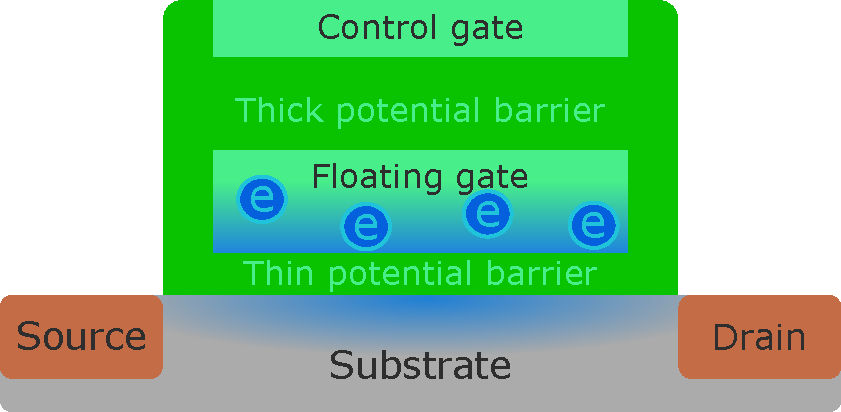
\includegraphics[width=0.5\textwidth]{figures/flash_memory.pdf}
	\caption{Schematic structure of a flash memory cell}
	\label{fig:flash_memory}
\end{figure}
For the writing and flushing to be possible, the thickness and height of the oxide layer --consequently, the potential wall-- between the floating gate and the substrate must be chosen carefully.
This barrier must be thick enough to prevent unwanted tunneling when no voltage is applied to the control gate.
After the control gate fills with electrons, the Coulomb potential created by those electrons makes an overall slope in the potential barrier created by the oxide layer.
The potential level inside the floating gate does not acquire a slope since it is made out of conducting material, hence its equipotential.
This slope is added to the potential barrier, thus changing its shape.
The previously rectangular barrier now acquired a triangular outline. More importantly, the $d$ width of the barrier gets reduced.
This increases the probability of the electron in the floating gate to tunnel out from the gate through the thin oxide layer into the substrate.
This phenomenon is called Fowler–Nordheim tunneling \cite{Fowler_1928bv}.
Figure \ref{fig:fowler_nordheim_tunneling} visualizes the principle of this effect.
\begin{figure}
	\centering
	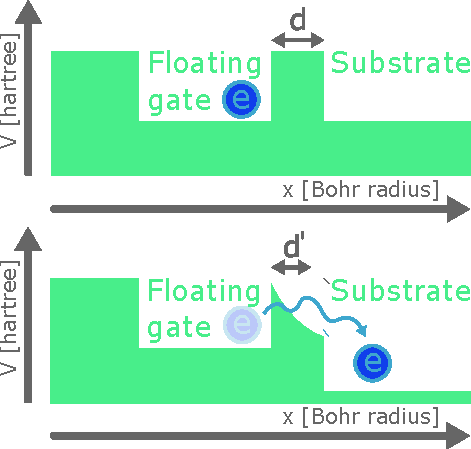
\includegraphics[width=0.5\textwidth]{figures/fowler_nordheim_tunneling.pdf}
	\caption{Fowler-Nordheim tunneling: on the upper image there is no Coulomb potential; on the image below Coulomb potential changes the shape of potential barrier causing tunneling}
	\label{fig:fowler_nordheim_tunneling}
\end{figure}
In our flash memory cell simulation, we initialized a potential wall representing the barrier between the floating gate and the substrate.
Our simulation deals with only one electron.
To simulate the flushing of the gate, we initialize the location of this electron to be inside the floating gate.
We add a Coulomb potential that decreases inside the thin oxide layer towards the substrate.
We initialized the barrier with a height of $V_0 = 10$ hartree and width of $d = 4.0$ Bohr radius.
We surrounded the floating gate area with thick potential barriers from the remaining five sides to prevent tunneling in unwanted directions. However, we excluded these from the visualization to make the electron's probability density visible from the outside.
We model the charge on the control gate as a uniformly charged infinite sheet.
This way, the Coulomb potential induced by a negatively charged control gate acting on an electron inside the oxide can be described by the following formula
\begin{equation}
	\label{eq:coulomb_potential}
	V_C = \frac{\sigma}{2r\epsilon}
\end{equation}
where $\epsilon$ is the dielectric permittivity of the oxide, $\sigma$ is the surface charge density at the control gate, and $r$ is the distance from the control gate.

We ran the simulation with the Coulomb potential turned on and off and compared the \textit{probability evolution} plots.
Figure \ref{fig:flash_flush_plot} shows the flushing of the floating gate with the Coulomb potential enabled.
The probability of the electron being found on the gate is decreasing.
\begin{figure}
	\centering
	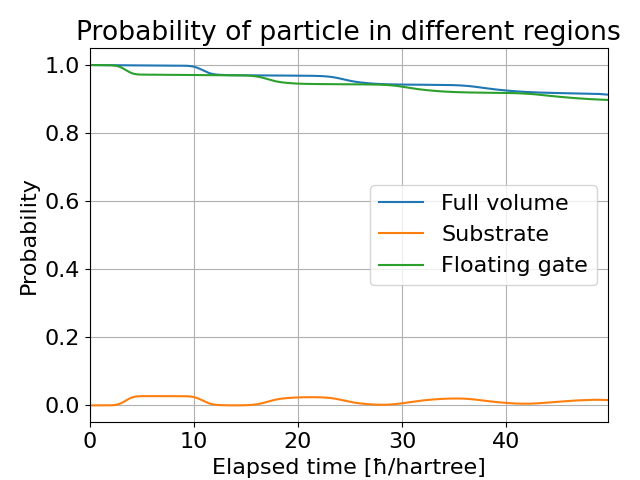
\includegraphics[width=0.6\textwidth]{figures/flash_flush.png}
	\caption{Flushing of the floating gate}
	\label{fig:flash_flush_plot}
\end{figure}
In figure \ref{fig:flash_keep}, however, the electron stays on the gate since we disabled the Coulomb potential.
\begin{figure}
	\centering
	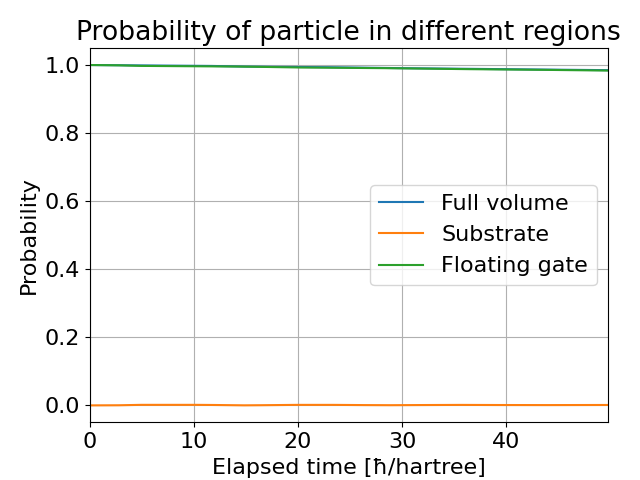
\includegraphics[width=0.6\textwidth]{figures/flash_keep.png}
	\caption{Storing the electron on the floating gate over a longer period of time}
	\label{fig:flash_keep}
\end{figure}
We also provide ray-traced visualization of the flash memory cell simulation.
This can be observed in figure \ref{fig:flash_memory_ray_traced} and in animation form on \url{} \todo{No URL}.

\todo{No figure about ray traced flash cell}





	\section{Discussion}
\label{sec:discussion}

In our work, we wrote about simulating the time development of the quantum mechanical wave function in 3D space.
Our accomplishments are the following
\begin{itemize}
	\item We adopted a simulation method that uses the Fourier transform as a subroutine to efficiently calculate the solution of the time-dependent Schrödinger equation.
	\item As an improvement over Géza István Márk's implementation, we ported the Fast Fourier Transform to the Graphical Programming Unit, thus reaching a major speed-up of a factor of 50 for some cases.
	\item We implemented the draining potential technique to allow longer simulation scenarios without the forming of unrealistic reflections and interference patterns.
	\item We combined state-of-the-art volume visualization techniques to enhance the visual quality of the resulting probability density images.
	\item We used multiple alternatives to visualize the probability densities, including \textit{canvas probability density}, good for visualizing diffraction, the \textit{per axis} approach that is handy when we do configuration space simulations or the \textit{probability evolution} used in the flash memory simulation.
	\item We used our simulator software to run various Wave Packet Dynamical simulations ranging from basic diffraction scenarios through simulation of lower dimensional particles in configuration space up to a more advanced case of simulating the writing and flushing sequence of a flash memory cell. For some of these scenarios, we provided analytical validation methods such as the one for the interference pattern of the double-slit experiment, the easily testable periodic time of the harmonic oscillator, or even the probability of the wave packet tunneling through barriers.
\end{itemize}
We see our work as a successful entry into the world of quantum mechanical wave packet dynamics and a definitely good starting point for further research.
We believe that the vast amount of application of quantum mechanics speaks for itself when the question is whether this research is important or not.
Another motivation to do wave packet dynamical simulations is the Nobel prize winning research of Dr. Ferenc Krausz. Attosecond physics opens a new frontier in understanding our universe.
Doing computer simulations and comparing the results with laboratory experiments can be a powerful strategy to make new discoveries.
We already have multiple ideas on how to improve and append the current method.
One obvious direction for development is to improve the user interface and to create a graphical interface besides the current terminal-based interface.
In the future, we want to make it possible to calculate the eigenstates of the localized potential.
This would require the calculation of the Fourier transform in the time domain to obtain the energy state of the system.
Then, iteratively converge towards the eigenstate.
There is also a possibility to incorporate electromagnetism into the Hamiltonian operator.
We have simulation 1D particles in
Making this work would also be a very exciting project.
From a visualization point of view, there are also many possibilities to improve.
As seen in this work, there is room for even better reconstruction filters
and clever ways to use the limited resolution.
We are very hopeful about the future research potential of this topic and are very eager to continue the fruitful work.



	

	\section{Acknowledgement}

I would like to thank my advisor, Dr. Balázs Csébfalvi, who has always been very supportive and open towards my silly ideas. One such ideas of mine was to begin to work with wave packet simulation.
I am immensely grateful for the work of Dr. Géza István Márk and Dr. Péter Vancsó as my supervisors and as first hand sources about wave packet dynamics.
Without their help this work wouldn't exist.
I would like to mention Dr. János Asbóth who recommended to look into the work of Dr. Géza I. Márk's work.
Basically he gave the first quantitative impulse to this research.



	

	\printglossaries

	\bibliography{references.bib}
	
\end{document}